%%%%%%%%%%%%%%%%%%%%%%%%%%%%%%%%%%%%%%%%%
% Classicthesis Typographic Thesis
% LaTeX Template
% Version 1.4 (1/1/16)
%
% This template has been downloaded from:
% http://www.LaTeXTemplates.com
%
% Original author:
% André Miede (http://www.miede.de) with commenting modifications by:
% Vel (vel@LaTeXTemplates.com)
%
% License:
% GNU General Public License (v2)
%%%%%%%%%%%%%%%%%%%%%%%%%%%%%%%%%%%%%%%%%

\documentclass[
		twoside,titlepage,headinclude,
	 	footinclude=true,cleardoublepage=empty,dottedtoc,
		BCOR=5mm,paper=a4,fontsize=11pt,
		ngerman,american,polish]{scrreprt}
%%%%%%%%%%%%%%%%%%%%%%%%%%%%%%%%%%%%%%%%%
% Classicthesis Typographic Thesis
% Configuration File
%
% This file has been downloaded from:
% http://www.LaTeXTemplates.com
%
% Original author:
% André Miede (http://www.miede.de) with extensive commenting changes by:
% Vel (vel@LaTeXTemplates.com)
%
% License:
% GNU General Public License (v2)
%
% Important note:
% The main lines to change in this file are in the DOCUMENT VARIABLES
% section, the rest of the file is for advanced configuration.
%
%%%%%%%%%%%%%%%%%%%%%%%%%%%%%%%%%%%%%%%%%

%----------------------------------------------------------------------------------------
%	CHARACTER ENCODING
%----------------------------------------------------------------------------------------

\PassOptionsToPackage{utf8}{inputenc} % Set the encoding of your files. UTF-8 is the only sensible encoding nowadays. If you can't read äöüßáéçèê∂åëæƒÏ€ then change the encoding setting in your editor, not the line below. If your editor does not support utf8 use another editor!
\usepackage{inputenc}

%----------------------------------------------------------------------------------------
%	DOCUMENT VARIABLES
%	Fill in the lines below to enter your information into the thesis template
%	Each of the commands can be cited anywhere in the thesis
%----------------------------------------------------------------------------------------

% Remove drafting to get rid of the '[ Date - classicthesis version 4.0 ]' text at the bottom of every page
\PassOptionsToPackage{eulerchapternumbers,listings,drafting, pdfspacing, subfig,beramono,eulermath,parts}{classicthesis}
% Available options: drafting parts nochapters linedheaders eulerchapternumbers beramono eulermath pdfspacing minionprospacing tocaligned dottedtoc manychapters listings floatperchapter subfig

\newcommand{\myTitle}{Algorytmy tekstowe\xspace}
\newcommand{\mySubtitle}{\xspace}
%\newcommand{\myDegree}{Doktor-Ingenieur (Dr.-Ing.)\xspace}
\newcommand{\myName}{Krzysztof Turowski\xspace}
\newcommand{\myFaculty}{Wydział Matematyki i Informatyki\xspace}
\newcommand{\myDepartment}{Instytut Informatyki Analitycznej\xspace}
\newcommand{\myUni}{Uniwersytet Jagielloński\xspace}
\newcommand{\myLocation}{Gdańsk-Kraków\xspace}
\newcommand{\myTime}{Semestr letni 2019/2020\xspace}
\newcommand{\myVersion}{wersja 1.0\xspace}

%----------------------------------------------------------------------------------------
%	USEFUL COMMANDS
%----------------------------------------------------------------------------------------

\newcommand{\ie}{i.\,e.}
\newcommand{\Ie}{I.\,e.}
\newcommand{\eg}{e.\,g.}
\newcommand{\Eg}{E.\,g.} 

\newcounter{dummy} % Necessary for correct hyperlinks (to index, bib, etc.)
\providecommand{\mLyX}{L\kern-.1667em\lower.25em\hbox{Y}\kern-.125emX\@}
\newlength{\abcd} % for ab..z string length calculation

% Different types of paragraph breaks
\newcommand{\pbn}{\par\bigskip\noindent}
\newcommand{\psn}{\par\smallskip\noindent}
\newcommand{\pn}{\par\noindent}

% Various notations
\newcommand{\E}{\mathbb{E}}
\newcommand{\Var}{\mathrm{Var}}
\newcommand{\cN}{\mathcal{N}}
\newcommand{\N}{\mathbb{N}}
\renewcommand{\Re}{\mathbb{R}}
\newcommand{\rank}[1]{\ensuremath{\textrm{rank}({#1})}}

% Function names with hyphens
\mathchardef\mhyphen="2D
\newcommand{\getmin}{get\mhyphen min}
\newcommand{\removemin}{remove\mhyphen min}
\newcommand{\decreasekey}{decrease\mhyphen key}
\newcommand{\insertfront}{insert\mhyphen front}

%----------------------------------------------------------------------------------------
%	PACKAGES
%----------------------------------------------------------------------------------------

\usepackage{lipsum}
\usepackage{todonotes}
\usepackage{algorithm}
\usepackage[noend]{algpseudocode}
\usepackage{mathtools}
\usepackage{enumitem}

\algdef{SE}[DOWHILE]{Do}{doWhile}{\algorithmicdo}[1]{\algorithmicwhile\ #1}

%------------------------------------------------			
\usepackage{csquotes}
\PassOptionsToPackage{%
%backend=biber, % Instead of bibtex
backend=bibtex8,bibencoding=ascii,%
language=auto,%
%style=numeric-comp,%
style=authoryear-comp, % Author 1999, 2010
%bibstyle=authoryear,dashed=false, % dashed: substitute rep. author with ---
sorting=ynt, % name, year, title
maxbibnames=10, % default: 3, et al.
%backref=true,%
natbib=true % natbib compatibility mode (\citep and \citet still work)
}{biblatex}
\usepackage{biblatex}

 %------------------------------------------------

\PassOptionsToPackage{fleqn}{amsmath} % Math environments and more by the AMS 
\usepackage{amsmath,amsthm,amsfonts,amssymb}

\theoremstyle{plain}
\newtheorem{theorem}{Theorem}[chapter]
\newtheorem{corollary}{Corollary}[chapter]
\newtheorem{lemma}[theorem]{Lemma}
\newtheorem{proposition}[theorem]{Proposition}
\theoremstyle{remark}
\newtheorem{remark}{Remark}[chapter]
\theoremstyle{definition}
\newtheorem{definition}{Definition}[chapter]
\newtheorem{problem}{Problem}[chapter]
\newtheorem{open_problem}[problem]{Open problem}

%------------------------------------------------

\PassOptionsToPackage{polish}{babel}
\usepackage{babel}
 
 %------------------------------------------------

\PassOptionsToPackage{T1}{fontenc} % T2A for cyrillics
\usepackage{fontenc}

%------------------------------------------------

\usepackage{textcomp} % Fix warning with missing font shapes

%------------------------------------------------

\usepackage{scrhack} % Fix warnings when using KOMA with listings package  

%------------------------------------------------

\usepackage{xspace} % To get the spacing after macros right

%------------------------------------------------

\usepackage{mparhack} % To get marginpar right

%------------------------------------------------

\PassOptionsToPackage{smaller}{acronym} % Include printonlyused in the first bracket to only show acronyms used in the text
\usepackage{acronym} % Nice macros for handling all acronyms in the thesis

%\renewcommand*{\acsfont}[1]{\textssc{#1}} % For MinionPro
\renewcommand*{\aclabelfont}[1]{\acsfont{#1}}

%------------------------------------------------

\PassOptionsToPackage{pdftex}{graphicx}
\usepackage{graphicx} 

%----------------------------------------------------------------------------------------
%	FLOATS: TABLES, FIGURES AND CAPTIONS SETUP
%----------------------------------------------------------------------------------------

\usepackage{tabularx} % Better tables
\setlength{\extrarowheight}{3pt} % Increase table row height
\newcommand{\tableheadline}[1]{\multicolumn{1}{c}{\spacedlowsmallcaps{#1}}}
\newcommand{\myfloatalign}{\centering} % To be used with each float for alignment
\usepackage{caption}
\captionsetup{font=small}
\usepackage{subfig}  

%----------------------------------------------------------------------------------------
%	CODE LISTINGS SETUP
%----------------------------------------------------------------------------------------

\usepackage{listings} 
%\lstset{emph={trueIndex,root},emphstyle=\color{BlueViolet}}%\underbar} % For special keywords
\lstset{language=[LaTeX]Tex,%C++ % Specify the language(s) for listings here
morekeywords={PassOptionsToPackage,selectlanguage},
keywordstyle=\color{RoyalBlue}, % Add \bfseries for bold
basicstyle=\small\ttfamily, % Makes listings a smaller font size and a different font
%identifierstyle=\color{NavyBlue}, % Color of text inside brackets
commentstyle=\color{Green}\ttfamily, % Color of comments
stringstyle=\rmfamily, % Font type to use for strings
numbers=left, % Change left to none to remove line numbers
numberstyle=\scriptsize, % Font size of the line numbers
stepnumber=5, % Increment of line numbers
numbersep=8pt, % Distance of line numbers from code listing
showstringspaces=false, % Sets whether spaces in strings should appear underlined
breaklines=true, % Force the code to stay in the confines of the listing box
%frameround=ftff, % Uncomment for rounded frame
%frame=single, % Frame border - none/leftline/topline/bottomline/lines/single/shadowbox/L
belowcaptionskip=.75\baselineskip % Space after the "Listing #: Desciption" text and the listing box
}

%----------------------------------------------------------------------------------------
%	HYPERREFERENCES
%----------------------------------------------------------------------------------------

\PassOptionsToPackage{pdftex,hyperfootnotes=false,pdfpagelabels}{hyperref}
\usepackage{hyperref}  % backref linktocpage pagebackref
\pdfcompresslevel=9
\pdfadjustspacing=1

\hypersetup{
% Uncomment the line below to remove all links (to references, figures, tables, etc), useful for b/w printouts
%draft, 
colorlinks=true, linktocpage=true, pdfstartpage=3, pdfstartview=FitV,
% Uncomment the line below if you want to have black links (e.g. for printing black and white)
%colorlinks=false, linktocpage=false, pdfborder={0 0 0}, pdfstartpage=3, pdfstartview=FitV, 
breaklinks=true, pdfpagemode=UseNone, pageanchor=true, pdfpagemode=UseOutlines,%
plainpages=false, bookmarksnumbered, bookmarksopen=true, bookmarksopenlevel=1,%
hypertexnames=true, pdfhighlight=/O,%nesting=true,%frenchlinks,%
urlcolor=webbrown, linkcolor=RoyalBlue, citecolor=webgreen, %pagecolor=RoyalBlue,%
    %urlcolor=Black, linkcolor=Black, citecolor=Black, %pagecolor=Black,%
%------------------------------------------------
% PDF file meta-information
pdftitle={\myTitle},
pdfauthor={\textcopyright\ \myName},
pdfsubject={},
pdfkeywords={},
pdfcreator={pdfLaTeX},
pdfproducer={LaTeX with hyperref and classicthesis}
%------------------------------------------------
}

%----------------------------------------------------------------------------------------
%	AUTOREFERENCES SETUP
%	Redefines how references in text are prefaced for different 
%	languages (e.g. "Section 1.2" or "section 1.2")
%----------------------------------------------------------------------------------------

\makeatletter
\@ifpackageloaded{babel}
{
\addto\extrasamerican{
\renewcommand*{\figureautorefname}{Figure}
\renewcommand*{\tableautorefname}{Table}
\renewcommand*{\partautorefname}{Part}
\renewcommand*{\chapterautorefname}{Chapter}
\renewcommand*{\sectionautorefname}{Section}
\renewcommand*{\subsectionautorefname}{Section}
\renewcommand*{\subsubsectionautorefname}{Section}
}
\addto\extrasngerman{
\renewcommand*{\paragraphautorefname}{Absatz}
\renewcommand*{\subparagraphautorefname}{Unterabsatz}
\renewcommand*{\footnoteautorefname}{Fu\"snote}
\renewcommand*{\FancyVerbLineautorefname}{Zeile}
\renewcommand*{\theoremautorefname}{Theorem}
\renewcommand*{\appendixautorefname}{Anhang}
\renewcommand*{\equationautorefname}{Gleichung}
\renewcommand*{\itemautorefname}{Punkt}
}
\providecommand{\subfigureautorefname}{\figureautorefname} % Fix to getting autorefs for subfigures right
}{\relax}
\makeatother

%----------------------------------------------------------------------------------------

\usepackage{classicthesis}
\usepackage[
    type={CC},
    modifier={by},
    version={4.0},
]{doclicense}

%----------------------------------------------------------------------------------------
%	CHANGING TEXT AREA 
%----------------------------------------------------------------------------------------

%\usepackage[showframe, pass]{geometry}
\areaset[current]{411pt}{761pt}
\setlength{\marginparwidth}{72pt}%
\setlength{\marginparsep}{0em}%
\setlength{\oddsidemargin}{20pt}%
\setlength{\evensidemargin}{0pt}%
\setlength{\hoffset}{11pt}%

%----------------------------------------------------------------------------------------
%	USING DIFFERENT FONTS
%----------------------------------------------------------------------------------------

%\usepackage[oldstylenums]{kpfonts} % oldstyle notextcomp
%\usepackage[osf]{libertine}
%\usepackage[light,condensed,math]{iwona}
%\renewcommand{\sfdefault}{iwona}
%\usepackage{lmodern} % <-- no osf support :-(
%\usepackage{cfr-lm} % 
%\usepackage[urw-garamond]{mathdesign} <-- no osf support :-(
%\usepackage[default,osfigures]{opensans} % scale=0.95 
%\usepackage[sfdefault]{FiraSans}


\addbibresource{bibliography/bibliography.bib}

%\hyphenation{Put special hyphenation here}

\begin{document}

\frenchspacing
\raggedbottom
\selectlanguage{polish}
\renewcommand*{\bibname}{References}
\pagenumbering{roman}
\pagestyle{plain}

\begin{titlepage}

\begin{addmargin}[0pt]{31pt}
\begin{center}
\Large
\hfill
\vfill
\begingroup
\color{Maroon}\spacedallcaps{\myTitle} \\ \bigskip % Thesis title
\endgroup
\spacedlowsmallcaps{\myName}
\vfill
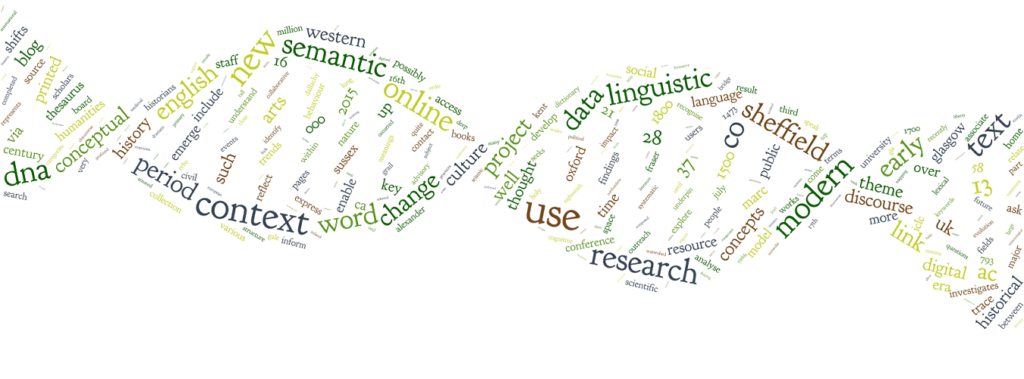
\includegraphics[width=12.5cm]{graphics/titlepage.png} \\
\vfill
\myTime\ -- \myVersion
\vfill
{\normalsize\doclicenseThis}
\end{center}
\end{addmargin}

\end{titlepage}

%%% % Back of the title page

\thispagestyle{empty}

\hfill

\vfill

\noindent\myName: \textit{\myTitle,} %\mySubtitle, %\myDegree, 
\textcopyright\ \myTime

\doclicenseThis

% You may wish to do something with the back of the title page, such as including your supervisors, location or time frame of the work. Below is an example of doing so although you may want to tweak it to your liking.

%\bigskip

%\noindent\spacedlowsmallcaps{Supervisors}: \\
%\myProf \\
%\myOtherProf \\ 
%\mySupervisor

%\medskip \\

%\noindent\spacedlowsmallcaps{Location}: \\
%\myLocation

%\medskip \\

%\noindent\spacedlowsmallcaps{Time Frame}: \\
%\myTime


%%% \cleardoublepage\thispagestyle{empty}
\refstepcounter{dummy}

\pdfbookmark[1]{Dedication}{Dedication}
\vspace*{3cm}

\begin{center}
\emph{Ohana} means family. \\
Family means nobody gets left behind, or forgotten. \\ \medskip
--- Lilo \& Stitch    
\end{center}

\medskip

\begin{center}
Dedicated to the loving memory of Rudolf Miede. \\ \smallskip
1939\,--\,2005
\end{center} % Dedication page

%%% \cleardoublepage\include{front-back/Foreword} % Uncomment and create a Foreword.tex to include a foreword

%%% \cleardoublepage\pdfbookmark[1]{Podziękowania}{Podziękowania}

\begin{flushright}{\slshape    
Jeśli widzę dalej, to tylko dlatego,
że stoję na ramionach olbrzymów.} \\ \medskip
--- Isaac Newton
\end{flushright}

\bigskip

\begingroup

\let\clearpage\relax
\let\cleardoublepage\relax
\let\cleardoublepage\relax

\chapter*{Podziękowania}

\noindent
Katarzyna Rajtar -- Masek, Paterson Algorithm Computing String Edit Distances
Mateusz Kaczmarek -- Approximate Boyer Moore
Mateusz Tokarz - Approximate shortest superstring within log
Wojciech Grabis -- Myers longest common subsequence algorithm
Mateusz Pabian -- Add fast practical multi pattern matching
Bartłomiej Jachowicz -- Kumar Rangan linear space lcs
Weronika Grzybowska -- IS suffix array 
Pawe\l Mader -- Landau-Vishkin string matching with k mismatches
Micha\l Zwonek - 3-Approximation of Shortest Superstrings 
Kamil Rajtar -- FFT exact string matching with wildcards
Pawe\l Palenica -- Larsson-Sadakane suffix array
Jan H\'avranek -- Manber-Myers suffix array queries
Adrian Siwiec -- Turbo Boyer-Moore exact string matching
Rafa\l Byczek -- Commentz-Walter exact multiple string matching
Piotr Miko\l{}ajczyk -- Aho-Corasick exact multiple string matching
Filip Bartodziej -- Ko-Aluru small-large suffix array
Bartosz Wodzi\'nski -- Farach suffix tree
Gabriela Czarska -- ??? optimal string matching

Bruno Pitrus -- Galil, Seiferas time-space optimal string matching

\endgroup % Acknowledgements page

\pagestyle{scrheadings}
\cleardoublepage
\refstepcounter{dummy}

\pdfbookmark[1]{\contentsname}{tableofcontents}

\setcounter{tocdepth}{2}
\setcounter{secnumdepth}{3}

\manualmark
\markboth{\spacedlowsmallcaps{\contentsname}}{\spacedlowsmallcaps{\contentsname}}
\tableofcontents 
\automark[section]{chapter}
\renewcommand{\chaptermark}[1]{\markboth{\spacedlowsmallcaps{#1}}{\spacedlowsmallcaps{#1}}}
\renewcommand{\sectionmark}[1]{\markright{\thesection\enspace\spacedlowsmallcaps{#1}}}

\clearpage

\begingroup 
\let\clearpage\relax
\let\cleardoublepage\relax
\let\cleardoublepage\relax

\endgroup
\cleardoublepage
\chapter{Wprowadzenie}

\section{Podstawowe pojęcia}

\begin{definition}{}{}
  \textbf{\textit{Alfabet}} $\A$ -- (skończony) zbiór symboli.
\end{definition}

W większości algorytmów rozmiar alfabetu jest stały i pomijany w analizie złożoności.

\begin{definition}{}{}
  \textbf{\textit{Słowo}} $w \in \A^*$ to ciąg symboli zbudowany nad alfabetem $\A$.
\end{definition}

Słowo puste jest oznaczane symbolem $\varepsilon$. Zbiór słów niepustych to $\A^+ = \A^* \setminus \{\varepsilon\}$.
Zbiór słów długości $n$ oznaczamy $\A_n$ i definiujemy rekurencyjnie jako $\A_0 = \{\varepsilon\}$, $A_{n + 1} = \bigcup_{x \in \A_n, y \in \A} xy$. 

Numerację symboli w słowie zaczynamy od $1$, więc $w[i]$ (albo $w_i$) jest $i$-tym symbolem w słowie $w$.

\begin{definition}{}{}
  \textbf{\textit{Długość słowa}} to funkcja $|\cdot|: \A^* \to \N$  taka, że $|w| = n$ wtedy i tylko wtedy, gdy $w \in \A_n$.
\end{definition}

\begin{definition}{}{}
  Słowo $u$ jest \textbf{\textit{podsłowem}} (ang. \emph{factor}) słowa $w$, gdy istnieją słowa $v_1 v_2 \in \A^*$ takie, że $w = v_1 u v_2$.
  Podsłowo jest \textbf{\textit{właściwe}}, gdy $v_1 v_2 \neq \varepsilon$.
\end{definition}

% Zbiór wszystkich podsłów oznaczamy $F(w) = \{u: \exists_{v_1, v_2: v_1 v_2\neq\varepsilon} v_1 u v_2\}$.
% Zbiór podsłów długości $k$ oznaczamy $F_k(w) = \{u: u \in F(w) \land |u| = k\}$.

\begin{definition}{}{}
  Słowo $u$ jest \textbf{\textit{prefiksem}} (\textbf{\textit{sufiksem}}) słowa $w$, gdy istnieje słowo $v \in \A^*$ takie, że $w = u v$ ($w = v u$).
  Prefiks (sufiks) jest \textbf{\textit{właściwy}}, gdy $v \neq \varepsilon$.
\end{definition}

\begin{definition}{}{}
  Słowo $u$ jest \textbf{\textit{podciągiem}} słowa $w$, gdy istnieją liczby $1 \le i_1 < i_2 < \ldots < i_k \le |w|$ takie, że $u = w[i_1] w[i_2] \ldots w[i_k]$.
\end{definition}

\begin{definition}{}{}
  Słowo $\bar{w}$ jest \textbf{\textit{odwrotnością}} słowa $w$, gdy dla $n = |w|$ mamy $\bar{w} = w[n] w[n - 1] \ldots w[1]$.
\end{definition}

\begin{definition}{}{}
  Słowo $w$ jest \textbf{\textit{palindromem}}, jeśli istnieją słowa $u, v \in \A^*$ takie, że $|u| \le 1$ i $w = \bar{v} u v$.
\end{definition}

\section{Porządki i odległości}

Złożoność obliczeniowa algorytmów tekstowych obliczana jest przy przyjęciu dwóch (binarnych) operacji atomowych na parach liter z alfabetu: $=$ oraz $\le$.

\begin{definition}{}{}
  Relacja $\preceq$ jest relacją \textbf{\textit{porządku prefiksowego}} tj. $u \preceq v$ wtedy i tylko wtedy, gdy $u$ jest prefiksem $u$.
\end{definition}

\begin{definition}{}{}
  Relacja $\preceq_R$ jest relacją \textbf{\textit{porządku wojskowego}} (\emph{radix}) tj. $u \preceq_R v$ wtedy i tylko wtedy, gdy:
  \begin{itemize}
    \item albo $|u| < |v|$,
    \item albo $|u| = |v|$ oraz istnieje $1 \le k \le |u|$ takie, że $u[k] < v[k]$ i dla wszystkich $1 \le j < k$ zachodzi $u[j] = v[j]$.
  \end{itemize}
\end{definition}

\begin{definition}{}{}
  Relacja $<$ jest relacją \textbf{\textit{porządku leksykograficznego}} tj. $u < v$ wtedy i tylko wtedy, gdy:
  \begin{itemize}
    \item albo $u$ jest prefiksem $v$,
    \item albo istnieje $1 \le k \le |u|$ takie, że $u[k] < v[k]$ i dla wszystkich $1 \le j < k$ zachodzi $u[j] = v[j]$.
  \end{itemize}
\end{definition}

\begin{corollary}{}{}
  Porządek leksykograficzny i wojskowy są porządkami liniowymi, rozszerzającymi porządek prefiksowy. Dla słów równego długości $u$, $v$ zachodzi $u < v$ wtedy i tylko wtedy, gdy $u \preceq_R v$.
\end{corollary}

\section{Okresy i słowa pierwotne}

\begin{definition}{}{}
  Liczba $p \in \N_+$ jest \textbf{\textit{okresem}} słowa $w$, jeśli dla każdego $1 \le i \le |w| - p$ zachodzi $w[i] = w[i + p]$.
  \\
  Najmniejszy okres słowa $w$ oznaczamy przez $p(w)$. Z definicji $|w|$ jest okresem słowa, więc $p(w)$ jest dobrze zdefiniowane.
\end{definition}

% Zbiór wszystkich okresów słowa $w$ oznaczamy przez $\Pi(w)$.

\begin{definition}{}{}
  Słowo $u$ jest \textbf{\textit{prefikso-sufiksem}} (ang. \emph{border}) słowa $w$, jeśli istnieją słowa $v_1, v_2$ takie, że $w = u v_1 = v_2 u$.
\end{definition}
Z definicji $\varepsilon$ jest prefikso-sufiksem każdego słowa $w$.

\begin{problem}{crochemore2002jewels}{s. 12}
  Pokaż, że następujące warunki są równoważne:
  \begin{enumerate}[label=(\roman*)]
    \item $w$ ma okres $p$,
    \item $w$ jest podsłowem pewnego $v^k$ dla $|v| = p$ i $k \ge 1$,
    \item $w = (uv)^kv$ dla $|uv| = p$, $v \neq \varepsilon$ i $k \ge 1$,
    \item $w$ ma prefikso-sufiks długości $|w| - p$.
  \end{enumerate} 
\end{problem}

\begin{definition}{}{}
  Słowo $w$ jest \textbf{\textit{pierwotne}}, jeśli nie istnieje słowo $v$ oraz liczba całkowita $k \ge 2$ takie, że $w = v^k$.
\end{definition}

\begin{problem}{lothaire2002algebraic}{Problem 1.2.1, s. 40}
  Słowo $w$ jest słowem pierwotnym wtedy i tylko wtedy, gdy $p(w) = |w|$ lub $p(w)$ nie dzieli $|w|$.
\end{problem}

\begin{problem}{lothaire2002algebraic}{Problem 8.1.6}
  Pokaż, że następujące twierdzenia są równoważne:
  \begin{enumerate}[label=(\roman*)]
    \item $p(w^2) = |w|$,
    \item $w$ jest słowem pierwotnym,
    \item $w^2$ zawiera dokładnie dwa wystąpienia $w$.
  \end{enumerate} 
\end{problem}

\begin{theorem-thm}[Słaby lemat o okresowości]
  Jeśli słowo $w$ ma okresy $p$ i $q$ takie, że $|w| \ge p + q$, to $w$ ma również okres $NWD(p, q)$.
\end{theorem-thm}

\begin{proof}
  Bez straty ogólności załóżmy, że $p \ge q$.
  Najpierw wykażemy, że jeżeli słowo $w$ ma okresy $p$ i $q$ oraz $|w| \ge p + q$, to $w$ ma również okres $p - q$.
  
  Dla $1 \le i \le q$ mamy $a[i] = a[i + p] = a[i + p - q]$, ponieważ $1 \le i \le i + p - q \ge i + p \le |w|$.
  Podobnie dla $q + 1 \le i \le |w| - (p - q)$ mamy $a[i] = a[i - q] = a[i + p - q]$, ponieważ $1 \le i - q \le i + p - q \ge |w|$.

  Z algorytmu Euklidesa wynika wprost, że iterując to rozumowanie możemy pokazać, że $w$ ma również okres $NWD(p, q)$.
\end{proof}

\begin{theorem-thm}[Silny lemat o okresowości]
  Jeśli słowo $w$ ma okresy $p$ i $q$ takie, że $|w| \ge p + q - NWD(p, q)$, to $w$ ma również okres $NWD(p, q)$.
\end{theorem-thm}

\begin{proof}%[\citealx{Theorem 8.1.4, s. 272}{lothaire2002algebraic}}]
  Po pierwsze, jeśli słowo $w$ ma okresy $0 < q < p \le |w|$, to prefiks i sufiks $w$ o długości $|w| - q$ mają okresy $p - q$.
  Dla prefiksu wystarczy zauważyć, że dla dowolnego $1 \le i \le |w| - p$ zachodzi $w[i] = w[i + p] = w[i + p - q]$ -- a to właśnie jest definicja okresu dla słowa $w[1..(|w| - q)]$. 

  Po drugie, jeśli $w$ ma okres $q$ i istnieje podsłowo $v$ słowa $w$ z $|v| \ge q$ takim, że $r$ jest okresem $v$ i $r$ dzieli $q$, to $w$ ma okres $r$.
  
  Niech $r = NWD(p, q)$. Dowód przebiega przez indukcję ze względu na $s = \frac{p + q}{r}$. Dla $p = q = r$ -- więc twierdzenie jest oczywiście spełnione np. dla $s = 2$.
  
  Dla $s > 2$ i $q < p$ weźmy słowo $w$ mające okresy $p$ i $q$ takie, że $|w| \ge p + q - r$. Niech $u = w[1..q]$ oraz $w = uv$. Wówczas z pierwszego faktu wiemy, że $v$ ma okres $p - q$.
  Jednocześnie $v$ jest podsłowem $w$ oraz $|v| = |w| - q \ge p - r \ge q$, więc $v$ ma również okres $q$.
  
  Dalej wiemy, że $r = NWD(p - q, q)$, $s > \frac{(p - q) + q}{r}$ oraz
  \begin{align*}
    |v| = |w| - q \ge (p + q - r) - q = (p - q) + q - NWD(p - q, q).
  \end{align*}
  Z założenia indukcyjnego $v$ ma zatem okres $r$. Ostatecznie z drugiego faktu wiemy, że $w$ ma też okres $r$.
\end{proof}

\begin{problem}{lothaire2002algebraic}{Remark 8.1.5, s. 272}
  Korzystając ze słów Fibonacciego pokaż, że warunku $|w| \ge p + q - NWD(p, q)$ w silnym lemacie o okresowości nie da się poprawić.
\end{problem}

\begin{definition}{}{}
  Liczba $ord(w)$ jest \textbf{\textit{rzędem}} słowa $w$, jeśli $ord(w) = |w|/p(w)$.
\end{definition}

\begin{problem}{}{}
  Pokaż, że słowo Fibonacciego jest słowem pierwotnym.
\end{problem}

\begin{proof}
Załóżmy, że istnieją $u, k: u^k = Fib_i, k > 1$. Wprowadźmy oznaczenie $u = st$ gdzie $s = u[1\ldots|u|-2]$ oraz $t = u[|u|-1,|u|]$. 

Na podstawie poprzedniego zadania wiemy, że słowa Fibonacciego bez ostatnich dwu znaków są palindromem. Dlatego $(st)^{k-1}s$ powinno też być palindromem. Z~tego wynika, że $s = \overline{s}$ oraz $t = \overline{t}$. To może zachodzić tylko dla dwu przypadków: $t = 00$ i $t = 11$. Na ćwiczeniach jednak zostało pokazane, że dla słów Fibonacciego jedyne dwie opcje są $t = 01$ i $t = 10$. Otrzymujemy sprzeczność, która pokazuje, że żadne słowo Fibonacciego nie można zapisać jako $u^k, k > 1$, więc każde słowo Fibonacciego jest słowem pierwotnym.
\end{proof}

\subsection{Słowa sprzężone}

\begin{definition}{}{}
  Słowa $v, w$ są \textbf{\textit{sprzężone}} wtedy i tylko wtedy, gdy istnieją słowa $u_1$, $u_2$ takie, że $v = u_1 u_2$ i $w = u_2 u_1$.
\end{definition}

\begin{corollary}{}{}
  Relacja sprzężenia (cyklicznego obrotu) jest relacją równoważności, więc definiuje klasy równoważności w $\A^*$.
\end{corollary}

\begin{problem}{lothaire2002algebraic}{}
  Pokaż, ile elementów ma klasa równoważności dla słowa $v$.
\end{problem}

\begin{problem}{crochemore2002jewels}{s. 17}
  Pokaż dowód małego twierdzenia Fermata na bazie wiedzy, że słowo pierwotne $v$ należy do klasy równoważności o mocy $|v|$.
\end{problem}

\begin{proof}
Przypomnijmy na wstępie dowodu wypowiedź małego twierdzenia Fermata: jeżeli $p$ jest liczbą pierwszą, a $n$ dowolną liczbą naturalną, to $p | (n^p-n)$.

Zdefiniujmy taką relację na słowach, że $x$ jest w relacji z $y$, jeżeli tylko $x$ jest cyklicznym przesunięciem $y$. Oczywiście jest to relacja równoważności. Rozważmy słowa unarne długości $p$, czyli słowa postaci $a^p$, gdzie $a$ jest pewną literą. Niech $K$ będzie zbiorem wszystkich nieunarnych słów długości $p$ nad alfabetem $\{1,\cdots,n\}$. Wszystkie te słowa są pierwotne, ponieważ ich długość jest liczbą pierwszą oraz nie są unarne. Na podstawie założeń dostajemy, że każda klasa równoważności naszej relacji ma dokładnie $p$ elementów. Dodatkowo zauważmy, że zbiór $K$ ma dokładnie $n^p-n$ elementów. Ponieważ $K$ może być podzielony na rozłączne podzbiory mające po $p$ elementów, to $p|(n^p-n)$, co kończy dowód.
\end{proof}

\begin{definition}{}{}
  Słowo $w$ jest \textbf{\textit{słowem Lyndona}} wtedy i tylko wtedy, gdy jest minimalnym (leksykograficznie, wojskowo) słowem w ramach klasy sprzężenia.
\end{definition}

\section{Morfizmy i klasy słów}

\begin{definition}{}{}
  Funkcja $f: \A^* \to \B^*$ jest \textbf{\textit{morfizmem}} (\textbf{\textit{podstawieniem}}) jeśli $f(xy) = f(x)f(y)$ dla wszystkich $x, y \in \A^*$.
\end{definition}
Morfizm jest dosłowny (\emph{literal}), gdy dla każdego $x \in \A$ zachodzi $|f(x)| = 1$. \\
Morfizm jest nieusuwający (\emph{non-erasing}), gdy dla każdego $x \in \A$ zachodzi $f(x) \neq \varepsilon$.

\subsection{Słowa Fibonacciego}

\begin{definition}{lothaire2002algebraic}{s. 10-11}
  Słowo $f_n$ jest \textbf{\textit{słowem Fibonacciego}}, gdy $f_0 = 0$, $f_1 = 01$ oraz $f_{k + 2} = f_{k + 1} f_k$ dla $k = 0, 1, \ldots$.
  \\
  Równoważnie, $f_k = \phi^n(0)$ dla morfizmu $\phi(0) = 01$, $\phi(1) = 0$.
\end{definition}

\begin{problem}{}{}
  Dla $k \ge 1$ niech $u = f_k f_{k + 1}$ i $v = f_{k + 1} f_k$. Pokaż, że $u$ powstaje z $v$ przez zamianę dwóch ostatnich liter.
\end{problem}

\begin{problem}{lothaire2002algebraic}{Problem 8.2.7, s. 308}
  Jeśli dla $u \in \A^+$ słowo $u^2$ jest podsłowem pewnego $f_k$, to $|u|$ jest pewną liczbą Fibonacciego i $u$ jest sprzężone z pewnym $f_l$.
\end{problem}

\subsection{Słowa Thuego-Morse'a}

\begin{definition}{lothaire2002algebraic}{s. 11}
  Słowo $u_n$ jest \textbf{\textit{słowem Thuego-Morse'a}}, gdy $u_0 = 0$, $v_0 = 1$ oraz $u_{k + 1} = u_k v_k$, $v_{k + 1} = v_k u_k$ dla $k = 0, 1, \ldots$.
  \\
  Równoważnie, $u_k = \mu^n(0)$ dla morfizmu $\mu(0) = 01$, $\mu(1) = 10$.
\end{definition}

\begin{problem}{}{}
  Udowodnić że słowa Thuego-Morse'a $u_n$ i $v_n$ są słowami pierwotnymi.
\end{problem}

\begin{proof}
Rozważmy ciąg $u_i$, $v_i$ z wykładu, który służył do definicji słów Thuego Morse'a. Pokażemy, że każde z słów $u_i, v_i$ jest pierwotne.
Oczywiście dla $i=0$, słowa $0$, $1$ są pierwotne.

Załóżmy teraz, że dla każdego $i < n$ wiemy, że $u_i, v_i$ są pierwotne. Pokażemy jak z tego wywnioskować, że $u_n$ jest pierwotne. Dowód dla $v_n$ jest zupełnie analogiczny, więc go pominiemy.

Zauważmy, że długość $u_n$ to $2^n$, czyli jeżeli $u^n = s^k$ to $|s| = \frac{2^n}{k}$. Jako, że $k$ to przynajmniej $2$ i dzieli $2^n$ to jest postaci $2^l$, gdzie $1 \leq l \leq n-1$. Z tego natychmiast wynika, że $s$ jest też okresem $u_{n-1}$ - sprzeczność.
\end{proof}

\begin{problem}{}{}
  Udowodnić że słowa Thuego-Morse'a $u_{2n}$ są palindromami.
\end{problem}

\begin{proof}
Zgodnie z definicją rekurencyjną mamy $u_0=0,v_0=1$ oraz $u_{k+1}=u_kv_k$, $v_{k+1}=v_ku_k$. Rozumować będziemy indukcyjnie. Dla $n=0$, słowo $u_0=0, v_0=1$ są oczywiście palindromami. Załóżmy zatem, że dla wszystkich $k < n$ prawdą jest, że $u_{2k}$ oraz $v_{2k}$ są palindromami. Będziemy chcieli wykazać, że jest to prawdą także dla $u_{2n}$ i $v_{2n}$. Z definicji rekurencyjnej dostajemy, że $u_{2n}=u_{2n-1}v_{2n-1}=u_{2n-2}v_{2n-2}v_{2n-2}u_{2n-2}$. Ponieważ $u_{2n_2}$ oraz $v_{2n-2}$ są palindromami na mocy założenia indukcyjnego, to $u_{2n}$ też jest palindromem. Dokładnie taki sam argument pokazuje, że $v_{2n}$ również jest palindromem. Zatem zakończyliśmy dowód kroku indukcyjnego, a więc też cały dowód.
\end{proof}

\begin{problem}{lothaire2002algebraic}{3.1.1, s. 113-114}
  Sprawdzić czy słowa Thuego-Morse'a zawierają podsłowa $u^3$ lub $(uv)^2u$ dla pewnych $u, v \in \A^+$.
\end{problem}

\section{Kody}

\begin{definition}{}{}
  $X \subset \A^+$ jest \textbf{\textit{kodem}}, gdy dla dowolnych $x_1, \ldots, x_n, y_1, \ldots, y_m \in X$ jeśli dla $x_1 \ldots x_n = y_1 \ldots y_m$, to $n = m$ oraz $x_i = y_i$ dla $i = 1, \ldots, n$.
\end{definition}

\begin{definition}{}{}
  $X \subset \A^+$ jest \textbf{\textit{kodem prefiksowym}} gdy $X$ jest kodem i dla żadnych $x, y \in X$ słowo $x$ nie jest prefiksem $y$.
\end{definition}

\begin{problem}{lothaire2002algebraic}{6.1.3, s. 198-199}
  Zbiór $X \subset A^{+}$ jest kodem dla $B^{*}$ wtedy i tylko wtedy, gdy dowolna bijekcja $f:\ X \rightarrow B$ indukuje iniekcyjny morfizm z $B^{*}$ na $A^{*}$.
\end{problem}

\begin{proof}
Rozważmy morfizm indukowany $\phi$. Niech
$$\phi(s_1s_2\dots s_n) = \phi(w_1s_2\dots w_m).$$ 
Czyli
$$\phi(s_1)\phi(s_2)\dots \phi(s_n) = \phi(w_1)\phi(w_2)\dots \phi(w_m),$$
zatem
$$f(s_1)f(s_2)\dots f(s_n) =  f(w_1)f(w_2)\dots f(w_n) \Leftrightarrow x_1 x_2\dots x_n = y_1 y_2 \dots y_n.$$
Skoro $x_i, y_j \in X$ i $X$ jest kodem to $n = m$, $x_i = y_i$ czyli z bijektywności $f$:
$$s_1s_2\dots s_n = w_1s_2\dots w_m,$$
czyli $\phi$ jest iniekcją.

Teraz dowiedziemy implikacji w drugą stronę:

Załóżmy, że $X$ nie jest kodem. Jeżeli istnieją $n < m$ oraz słowa $x_1, \dots, x_n, y_1, \dots, y_m \in X$ takie, że 
$$x_1 \dots x_n = y_1 \dots y_m,$$ 
to niech $f$ będzie dowolną bijekcją z $B$ w $X$ i $b_i = f^{-1}(x_i)$ oraz $a_j = f^{-1}(y_j)$. Słowa
$$a_1 \dots a_n \text{ oraz } b_1 \dots b_m$$
są różnej długości więc są różne. Równocześnie dla $\phi$ - morfizmu indukowanego przez $f$ zachodzi
$$\phi(a_1 \dots a_n) = x_1 \dots x_n = y_1 \dots y_m = \phi(b_1 \dots b_m),$$
czyli nie jest iniekcją - sprzeczność.

Jeżeli natomiast $n=m$ i $x_1, \dots, x_n, y_1, \dots, y_n \in X$ takie, że
$x_1 \dots x_n = y_1 \dots y_n$
oraz istnieje $i$ spełniające 
$x_i \neq y_i,$
to ponownie rozważamy dowolną bijekcję z $B$ w $X$ i $b_j = f^{-1}(x_j)$ oraz $a_j = f^{-1}(y_j)$.

Słowa
$a_1 \dots a_n \text{ oraz } b_1 \dots b_n$
są różne, bo $a_i \neq b_i$. Równocześnie dla $\phi$ -- morfizmu indukowanego przez $f$ zachodzi
$$\phi(a_1 \dots a_n) = x_1 \dots x_n = y_1 \dots y_n = \phi(b_1 \dots b_n),$$
czyli nie jest iniekcją - sprzeczność.
To kończy cały dowód.
\end{proof}

\cleardoublepage
\pagenumbering{arabic}
\cleardoublepage

\chapter{Dokładne dopasowanie wzorca}

\begin{algorithm}[H]
    \caption{Dokładne dopasowanie wzorca}
    \Input{Słowa $t, w \in \A^+$ ($|t| = n$, $|w| = m$)}
    \Output{\textsc{True} jeśli $w$ jest podsłowem $t$, \textsc{False} w przeciwnym przypadku}
\end{algorithm}

\begin{algorithm}[H]
    \caption{Wyszukiwanie wszystkich wystąpień wzorca w tekście}
    \Input{Słowa $t, w \in \A^+$ ($|t| = n$, $|w| = m$)}
    \Output{Zbiór liczb $S = \{1 \le i \le n: t[i..(i + m - 1)] = w\}$.}
\end{algorithm}

\section{Algorytm naiwny}

\begin{code}
\captionof{listing}{Naiwne szukanie wprzód wzorca $w$ w tekście $t$}
\inputminted{python}{code/exact-string-matching/naive-forward.py}
\label{alg:exact-string-matching-naive-forward}
\end{code}

\begin{problem}{}{}
  Dla ustalonego $n$ i $m$ znajdź przykład słowa $w$ i tekstu $t$ z $|t| = n$, $|w| = m$, dla którego \Cref{alg:exact-string-matching-naive-forward} wykonuje najwięcej porównań.
\end{problem}

\begin{proof}
Najprostszym przykładem jest poszukiwanie wzorca $w=a^{m-1}b$ w tekście $t=a^n$. Dla takiego zestawu algorytm naiwny nie znajdzie dopasowania, a wcześniej będzie dopasowywał prawie całe słowo $w$, rozpoczynając od każdej pozycji słowa $t$. Prowadzi to do wykonania dokładnie $m (n - m + 1)$ porównań.
\end{proof}

Można również zaimplementować algorytm naiwny, który dopasowywałby wzorzec do tekstu od końca.

\begin{code}
\captionof{listing}{Naiwne szukanie wspak wzorca $w$ w tekście $t$}
\inputminted{python}{code/exact-string-matching/naive-backward.py}
\label{alg:exact-string-matching-naive-backward}
\end{code}

\section{Algorytm Morrisa-Pratta}

Algorytm naiwny dokonuje w razie wykrycia niedopasowania przesunięcia wzorca tekstu o $1$.
Załóżmy, że zachodzi $t[i + k + 1] = w[k + 1]$ dla pewnego $k$ oraz $t[i + j] = w[j]$ dla $1 \le j \le k$ tj. mamy zgodność wzorca z tekstem na $k$ literach.

Jasne jest jednak, że jeśli $v$ nie jest prefikso-sufiksem $w[1..k]$, to istnieje pozycja $0 \le l \le k - 1$ taka, że $v[|v| - l] \neq w[k - l] = t[i + k - l]$ -- a zatem nie ma sensu dopasowywać $w$. Z kolei jeśli $v$ jest prefikso-sufiksem $w[1..k]$, to z góry wiemy, że jest zgodne z $t[(i + k - |v|)..(i + k)]$.

Wobec tego najmniejsze sensowne przesunięcie to przejście do sprawdzania dla największego prefikso-sufisku $w[1..k]$ -- czyli przesunięcie o $p(w[1..k])$.

Dla słowa $w$ można zdefiniować tablice najdłuższych prefikso-sufiksów dla każdego prefiksu:
\begin{align*}
  B[i] = 
  \begin{cases}
    -1 & \text{dla $i = 0$,} \\
    \max\{k \ge 0:\text{$w[1 \ldots k]$ jest właściwym sufiksem $w[1\ldots i]$}\} & \text{dla $1 \le i \le |w|$.}
  \end{cases}
\end{align*}

\begin{lemma}{}{}
  \label{lem:pref-suf}
  Jeśli $u$ jest prefikso-sufiksem $v$ i $v$ jest prefikso-sufiksem $w$, to $u$ jest prefikso-sufiksem $w$.
\end{lemma}

\begin{corollary}{}{}
  Ciąg $(B[|w|], B[B[|w|]], \ldots, 0)$ zawiera długości wszystkich prefikso-sufiksów słowa $w$ w kolejności malejącej.
\end{corollary}

\begin{corollary}{}{}
  Ciąg $(|w|, \ldots, |w| - B[B[|w|]], |w| - B[|w|])$ zawiera długości wszystkich okresów słowa $w$ w kolejności malejącej.
\end{corollary}

\begin{code}
\captionof{listing}{Tablica prefikso-sufiksów}
\inputminted{python}{code/other/prefix-suffix.py}
\label{alg:prefix-suffix}
\end{code}

\begin{problem}{crochemore2002jewels}{Lemma 3.1, s. 34-35}
  Pokaż, jaki dokładny pesymistyczny czas działania ma \Cref{alg:prefix-suffix}.
\end{problem}

%$2m-3$. Wynik osiągalny dla $pat = 010^{m-2}$.

\begin{code}
\captionof{listing}{Algorytm Morrisa-Pratta}
\inputminted{python}{code/exact-string-matching/morris-pratt.py}
\label{alg:exact-string-matching-morris-pratt}
\end{code}

\begin{problem}{}{}
  Pokaż, ile razy w najgorszym razie pojedynczy symbol tekstu $t$ może zostać porównany z wzorcem w Algorytmie \ref{alg:exact-string-matching-morris-pratt}.
\end{problem}

\begin{problem}{}{}
  Pokaż, ile dokładnie porównań wykonuje w najgorszym przypadku zmodyfikowany \Cref{alg:exact-string-matching-morris-pratt}, zwracający wszystkie wystąpienia (tj. pozycje indeksów początkowych) $w$ w $t$.
\end{problem}

\section{Algorytm Knutha-Morrisa-Pratta}

Przesunięcie o $p(w[1..k]) = k - B[k]$ nie musi być najlepsze możliwe. Jeśli niedopasowanie zaszło na znakach $t[i + k + 1] \neq w[j + 1]$ oraz wiadomo z analizy wzorca, że $w[k + 1] = w[k - p(w) + 1]$, to wiadomo, że nie znajdziemy wzorca przez przesunięcie tylko o $p(w)$. Za to możemy szukać prefikso-sufiksu $w'$ dla słowa $w[1..j]$ takiego, że następuje po nim znak inny niż $w[j + 1]$ -- czyli tzw. silnego prefikso-sufiksu.

Dla słowa $w$ można zdefiniować tablice silnych prefikso-sufiksów następująco:
\begin{align*}
  sB[i] = 
  \begin{cases}
    \max\{0 \le k < i:\text{$w[1 \ldots k]$ jest sufiksem $w[1\ldots i]$} & \text{dla $1 \le i \le |w| - 1$,} \\
    \qquad\qquad\quad\text{i $w[k + 1] = w[i + 1]$}\} \\
    B[i] & \text{dla $i = |w|$,} \\
    -1 & \text{w pozostałych przypadkach.}
  \end{cases}
\end{align*}

\begin{code}
\captionof{listing}{Tablica silnych prefikso-sufiksów}
\inputminted{python}{code/other/strong-prefix-suffix.py}
\label{alg:strong-prefix-suffix}
\end{code}

\begin{problem}{}{}
  Pokaż, jaki dokładny pesymistyczny czas działania ma \Cref{alg:strong-prefix-suffix}.
\end{problem}

%$3m-5$. Wynik osiągalny dla $pat = 010^{m-2}$.

\begin{code}
\captionof{listing}{Algorytm Knutha-Morrisa-Pratta}
\inputminted{python}{code/exact-string-matching/knuth-morris-pratt.py}
\label{alg:exact-string-matching-knuth-morris-pratt}
\end{code}

\begin{problem}{galil1997pattern}{}
  Pokaż, ile razy w najgorszym razie pojedynczy symbol tekstu $t$ może zostać porównany z wzorcem w Algorytmie \ref{alg:exact-string-matching-knuth-morris-pratt}.
\end{problem}

\begin{problem}{galil1997pattern}{}
  Pokaż, ile dokładnie porównań wykonuje w najgorszym przypadku zmodyfikowany \Cref{alg:exact-string-matching-knuth-morris-pratt}, zwracający wszystkie wystąpienia (tj. pozycje indeksów początkowych) $w$ w $t$.
\end{problem}

\section{Algorytm Boyera-Moore'a}

Algorytm Boyera-Moore'a polega na ulepszeniu naiwnego dopasowywania wzorca od prawej do lewej.
Schemat jest taki sam jak dla algorytmów Morrisa-Pratta i Knutha-Morrisa-Pratta: wykonujemy dopasowanie dla danej pozycji okna, w razie znalezienia niedopasowania przesuwamy okno o pewną wartość.

Sprawdzanie dopasowania wzorca od prawej do lewej umożliwia, żeby algorytm wykonał $O\left(\frac{m}{n}\right)$ porównań np. dla $t = 0^n$, $w = 0^{m - 1}1$. Wystarczy np. wiedzieć, że wzorzec nie jest okresowy tj. $p(w) = |w|$ oraz że zachodzi $t[i] \neq w[m]$, aby następne sprawdzanie rozpocząć od pozycji $i + m$. Zauważmy, że w algorytmie KMP zawsze musimy porównać każdą literę tekstu ze wzorcem.

W praktyce to powoduje, że algorytm Boyera-Moore'a jest zauważalnie szybszy niż KMP lub MP.

Sednem algorytmu Boyera-Moore'a są 2 niezmienniki:
\begin{itemize}
  \item $cond_1(j, s)$ -- dla każdego $j  < k \le m$ zachodzi $s \ge k$ lub $w[k - s] = w[k]$,
  \item $cond_2(j, s)$ -- dla $s < j$ zachodzi $w[j - s] \neq w[j]$.
\end{itemize}

Wówczas możemy zdefiniować tablicę $BM$ w następujący sposób:
\begin{align*}
  BM[j] =
  \begin{cases}
    \min \{s > 0: cond_1(j, s) \land cond_2(j, s)\} & \text{dla $1 \le j < m$}, \\
    p(w) & \text{dla $j \in \{0, m\}$}.
  \end{cases}
\end{align*}
Tablica ta, podobnie jak tablica silnych prefikso-sufiksów w algorytmie KMP, określa o ile możemy przesunąć wzorzec względem tekstu w razie niedopasowania -- tylko od końca.

Aby efektywnie obliczyć tablicę $BM$ będzie potrzebna tablica prefikso-prefiksów:
\begin{align*}
  PREF[j] =
  \begin{cases}
    \max \{s \ge 0: \text{$w[j:j + s - 1]$ jest prefiksem $w$}\} & \text{dla $1 \le j \le m$}, \\
    -1 & \text{dla $j = 0$}.
  \end{cases}
\end{align*}

\begin{code}
\captionof{listing}{Tablica prefiksowo-prefiksowa}
\inputminted{python}{code/other/prefix-prefix.py}
\label{alg:prefix-prefix}
\end{code}

\begin{theorem}{}{}
  Algorytm \ref{alg:prefix-prefix} wyznacza poprawną tablicę prefikso-prefiksów dla słowa $w$ długości $m$.
\end{theorem}

\begin{proof}
  Niech tablica $PREF$ będzie poprawnie wypełniona dla wszystkich $2 \le j < i$ oraz niech $1 \le s < i$ będzie wartością, dla której $s + PREF[s]$ jest maksymalne.
  Niech ponadto $s_{max} = s + PREF[s] - 1$, $k = i - s + 1$ oraz $r = PREF[k]$
  
  Wówczas mamy 3 sytuacje:
  \begin{enumerate}
      \item $s + PREF[s] < i$ -- wówczas obliczamy wartość $PREF[i]$ naiwnie porównując $w$ i $w[i:m]$,
      \item $s + PREF[s] \ge i$ oraz $PREF[k] + k - 1 < PREF[s]$ dla $k = i - s + 1$ -- wówczas z definicji $s$ wiemy, że $w[s:s_{max}] = w[1:(s_{max} - s + 1)]$ oraz $i \in [s, s_{max}]$ (z pierwszego) oraz $w[1:r] = w[k:(r + k - 1)]$, $w[r + 1] \neq w[r + k]$ (z drugiego), wobec czego również $w[1:r] = w[i:(r + i - 1)]$ i $w[r + 1] \neq w[r + i]$, a więc $PREF[i] = r$,
      \item $s + PREF[s] \ge i$ oraz $PREF[k] + k - 1 \ge PREF[s]$ dla $k = i - s + 1$ -- wówczas podobnie jak powyżej mamy $w[1:(s_{max} - i + 1)] = w[i:s_{max}]$, więc sprawdzamy wydłużanie zgodności, naiwnie porównując $w[s_{max} - i:m]$ oraz $w[s_{max} + 1:m]$.
  \end{enumerate}
\end{proof}

\begin{theorem}{}{}
  Algorytm \ref{alg:prefix-prefix} dla słowa długości $m$ działa w czasie $O(m)$.
\end{theorem}

\begin{proof}
  Wystarczy zauważyć, że w funkcji \texttt{naive\_scan} kolejne wartości $j + r$ w ramach wszystkich wywołań tworzą ciąg rosnący.
\end{proof}

\begin{code}
\captionof{listing}{Tablica maksymalnych sufiksów}
\inputminted{python}{code/other/maximum-suffixes.py}
\label{alg:maximum-suffixes}
\end{code}

\begin{code}
\captionof{listing}{Tablica przesunięć według dobrych sufiksów}
\inputminted{python}{code/other/boyer-moore-shift.py}
\label{alg:boyer-moore-shift}
\end{code}

\begin{problem}{}{}
  Pokaż, że Algorytm \ref{alg:boyer-moore-shift} poprawnie oblicza wartości tablicy $BM$ w czasie $O(m)$.
\end{problem}

% Fakt: jeśli $BM[j] = m - k < j$, to $S[k] = m - j$.

\begin{problem}{}{}
    Pokaż, jak policzyć tablicę $wBM = \min\{s > 0: cond_1(j, s)\}$ w czasie $O(m)$.
\end{problem}

\begin{code}
\captionof{listing}{Algorytm Boyera-Moore'a}
\inputminted{python}{code/exact-string-matching/boyer-moore.py}
\label{alg:exact-string-matching-boyer-moore}
\end{code}

\begin{problem}{crochemore2002jewels}{s. 41}
  Pokaż, że dla wszystkich $n$, $m$ istnieje tekst $t$ i wzorzec $w$ ($|t| = n$, $|w| = m$) takie, że wyszukanie wzorca $w$ w tekście $t$
  z użyciem algorytmu Boyera-Moore'a wymaga czasu $O(n + m)$ a dla algorytmu wykorzystującego tablicę $wBM = \min\{s > 0: cond_1(j, s)\}$ zamiast $BM$ wymaga czasu $\Omega(n m)$.
\end{problem}

%Odpowiedź: w = ca(ba)^k, t = a^{2k + 2}ba

\subsection{Znajdowanie wszystkich wystąpień wzorca}

Tak jak algorytm KMP, tak algorytm BM można łatwo zmodyfikować, by zwracał wszystkie wystąpienia wzorca w tekście. Wystarczy przyjąć, że $BM[0] = p(w)$.
\begin{problem}{}{}
  Pokaż, że jeśli tekst $t$ zawiera $r$ wystąpień wzorca $w$, to czas działania algorytmu Boyera-Moore'a wynosi $\Omega(r m)$.
\end{problem}

\begin{corollary}{}{}
  Jeśli wzorzec występuje w tekście $\Theta(n)$ razy, to czas działania algorytmu Boyera-Moore'a wynosi $\Omega(n m)$.
\end{corollary}

Rozwiązaniem jest wykorzystanie zmiennej $memory$, zawierającej numer pierwszego indeksu, którego nie musimy sprawdzać.
W większości obrotów pętli $memory = 0$, jedynym wyjątkiem jest sytuacja, gdy zaszło dopasowanie -- wtedy wiemy, że $m - p(w)$ pierwszych symboli już jest dopasowanych i wystarczy porównać $w[(m - p(w) + 1)..m]$ z tekstem.

\begin{code}
\captionof{listing}{Algorytm Boyera-Moore'a-Galila}
\inputminted{python}{code/exact-string-matching/boyer-moore-galil.py}
\label{alg:exact-string-matching-boyer-moore-galil}
\end{code}

\subsection{Dowód liniowej złożoności algorytmu}

\todo[inline]{Dowód Cole'a}

\begin{theorem}{}{}
  Algorytm \ref{alg:exact-string-matching-boyer-moore} wymaga $O(n' + m)$ czasu do stwierdzenia pierwszego wystąpienia wzorca $w$ z tekście $t$, gdy to wystąpienie zostało znalezione na pozycji $n'$.
\end{theorem}

\begin{corollary}{}{}
  Algorytm \ref{alg:exact-string-matching-boyer-moore} wymaga $O(n + m)$ czasu do stwierdzenia, czy słowo $t$ zawiera podsłowo $w$.
\end{corollary}

\begin{theorem}{}{}
  Algorytm \ref{alg:exact-string-matching-boyer-moore-galil} działa w czasie $O(n + m)$.
\end{theorem}

\begin{proof}
  Z poprzedniego twierdzenia łatwo wykazać, że znalezienie wszystkich wystąpień wymaga czasu $O(n + r m)$ dla $r$ wystąpień wzorca w tekście dla Algorytmu \ref{alg:exact-string-matching-boyer-moore}, a więc również dla Algorytmu \ref{alg:exact-string-matching-boyer-moore-galil}.
  
  Jeśli $p(w) \ge \frac{m}{2}$, to z faktu $r \le \frac{n}{p(w)}$ wynika, że całkowita złożoność wynosi $O(n)$.
  
  Jeśli $p(w) < \frac{m}{2}$, to możemy pogrupować wystąpienia wzorca jeśli dwa kolejne w ciągu są odległe o $p(w)$. W każdym takim łańcuchu w Algorytmie \ref{alg:exact-string-matching-boyer-moore-galil} przejrzymy każdy symbol w łańcuchu tylko raz.
  Jeśli natomiast wykryjemy niedopasowanie, to wiemy, że następne przesuniecie zgodnie z dobrym sufiksem wynosi $|w| - p(w) \ge \frac{m}{2}$. Wobec każdy symbol poza łańcuchami odczytamy co najwyżej $2$ razy, a zatem złożoność również będzie liniowa.
\end{proof}

\subsection{Heurystyka \emph{occurrence shift}}

W oryginalnym artykule Boyera i Moore'a zaproponowano również dodatkową heurystykę \emph{occurrence shift}, opartą na znajomości wystąpień liter z alfabetu we wzorcu.

Zdefiniujmy tablicę $LAST$ w następujący sposób:
\begin{align*}
  L[x] =
  \begin{cases}
    \max \{1 \le i \le m: w[i] = x \land \forall_{i < j \le m} w[j] \neq m\} & \text{gdy $x$ występuje w $w$}, \\
    0 & \text{w przeciwnym przypadku}.
  \end{cases}
\end{align*}
Jeśli wiemy, że niedopasowanie nastąpiło na $w[j] \neq t[i + j]$, to wiemy również, że nie ma sensu sprawdzać przesunięć krótszych niż $j - LAST[t[i + j]]$. Mówiąc prościej, jeśli $t[i + j] = x$ oraz $x$ występuje w $w$ najpóźniej na pozycji $k$ (tj. $k = LAST[t[i + j]]$), to mamy 2 sytuacje:
\begin{itemize}
  \item albo $k > j$, wtedy wiedza z tablicy $LAST$ nam nic nie pomaga,
  \item albo $k < j$, wtedy wiemy, że pierwszą okazją na znalezienie dopasowania jest zestawienie ze sobą $w[k]$ i $t[i + j]$ -- czyli właśnie przesunięcie o $j - k$.
\end{itemize}
Dla znanego, skończonego alfabetu widać wprost, że wyznaczenie tablicy $LAST$ wymaga czasu i pomięci $O(m + |\A|)$.

Ponieważ heurystyka nie wyklucza się z obserwacjami dokonanymi na bazie tablicy $BM$, jej zastosowanie polega na zastąpieniu przesunięć o $BM[j]$ przesunięciami o $\max\{BM[j], j - LAST[t[i + j]]\}$.

W praktyce heurystyka ma sens wtedy, gdy alfabety są większe, ale dla alfabetu binarnego jest mało skuteczna.
Co ciekawe, brakuje teoretycznych analiz skuteczności użycia tej heurystyki np. względem podstawowego algorytmu Boyera-Moore'a.

\begin{problem}{}{}
  Niech w Algorytmie \ref{alg:exact-string-matching-boyer-moore} w linii ??? będzie miał zamiast $i = i + BM[j]$ polecenie $i = i + \max\{1, j - LAST[t[i + j]]\}$.
  Pokaż dla dowolnych $n$ i $m$ przykłady słów $t$ i $w$ ($|t| = n$, $|w| = m$) takich, że zmodyfikowany algorytm wymaga $\Omega(n m)$ porównań.
\end{problem}

Ten sam pomysł pojawia się u Horspoola, który postanowił korzystać tylko z przesuwania o \emph{occurrence shift} zgodnie z ostatnim znakiem aktualnie przetwarzanego tekstu.

\begin{code}
\captionof{listing}{Algorytm Horspoola}
\inputminted{python}{code/exact-string-matching/horspool.py}
\label{alg:exact-string-matching-horspool}
\end{code}

\begin{problem}{}{}
  Pokaż dla dowolnych $n$ i $m$ przykłady słów $t$ i $w$ ($|t| = n$, $|w| = m$) takich, że algorytm Horspoola wymaga $\Omega(n m)$ porównań.
\end{problem}

Raita zaproponował dodatkowo, żeby zamiast przechodzić do porównania tekstu z wzorcem za każdym razem wykonać najpierw porównanie symbolu ostatniego, pierwszego i środkowego.
Uzasadniał to tym, że wyszukiwanie słów w językach naturalnych często natrafia na problem częstych sufiksów (np. w angielskim \emph{-ing}, \emph{-ion}, \emph{-ed}) \cite{raita1992tuning}, aczkolwiek dalsze eksperymenty na tekstach losowych również przyniosły podobne rezultaty, co sugeruje że korzyści mogą być spowodowane czymś innym \cite{smith1994tuning}.

\subsection{Quick search}

Można zaproponować również inną heurystykę opartą o \emph{occurrence shift}: jeśli zaszło niedopasowanie na fragmencie tekstu $t[(i - j)..(i - 1)]$, to wiemy, że następne porównanie tekstu z wzorcem będzie zawierało $t[i]$. Wobec tego można od razu przesunąć tekst tak, aby uzgodnić ostatnie wystąpienie litery $t[i]$ we wzorcu z tekstem.

\begin{code}
\captionof{listing}{Algorytm \emph{quick search}}
\inputminted{python}{code/exact-string-matching/quick-search.py}
\label{alg:exact-string-matching-quick-search}
\end{code}

Smith zauważył, że można połączyć podejście Horspoola i Quick Search tj. brać maksimum z obu zalecanych przesunięć, aby otrzymać praktyczne przyspieszenie algorytmu \cite{smith1991experiments}.

\section{Algorytm Turbo~BM}

Algorytm Turbo~BM jest modyfikacją algorytmu Boyera-Moore'a, która zużywa tylko stałą dodatkową pamięć oraz przyspiesza złożoność pesymistyczną do $2n$. Nie będziemy wykonywać żadnego dodatkowego przetwarzania wstępnego -- tak jak w oryginalnym algorytmie korzystać będziemy z tablicy $BM$ obliczonej dla wzorca.
  
Sam pomysł algorytmu Turbo~BM jest bardzo prosty -- podczas skanowania będziemy zapisywać jedno podsłowo wzorca (\emph{memory}), o którym wiemy że pasuje do tekstu na obecnej pozycji. Dzięki temu możemy pominąć ten fragment przy sprawdzaniu dopasowania, oraz w przypadku jego braku możemy wykonać tzw. \emph{Turbo-shift}.

Opiszmy sytuację, w której możemy wykonać Turbo-shift. Niech $x$ będzie najdłuższym sufiksem wzorca, który pasuje do tekstu na danej pozycji, $a$ będzie pierwszą literą wzorca która nie pasuje, a niech $y$ ($memory$) będzie poprzednio zapamiętanym podsłowem, które również pasuje do wzorca (patrz fig. \ref{turboshift}). Załóżmy również, że $x$ i $y$ są rozłączne i $y$ jest dłuższy od $x$. Po wykonaniu Turbo-shift zapominamy o $y$ (patrz kod \emph{boyer\_moore\_turbo}), więc w poprzednim kroku wykonaliśmy zwykłe przesunięcie (zgodnie z tablicą $BM$), znane z algorytmu Boyera-Moore'a. W tej sytuacji $ax$ jest suffixem $y$, oraz litery $a$ i $b$ tekstu są o siebie oddalone o $|y|$. Ale suffix $y\ldots x$ ma okres długości $|y|$ (z definicji $BM$). Możemy więc przesunąć wzorzec o $|y| - |x|$ do przodu i to właśnie przesunięcie nazywać będziemy \emph{Turbo-shift}.

\begin{figure}[h]
	\centering
	\begin{tikzpicture}
		\begin{scope}[shift={(0,0)}, start chain=1 going right,node distance=0mm]
			\node [on chain=1,tmtape, minimum width=1.2cm, dashed] {text};
			\node [on chain=1,tmtape, minimum width=1.1cm, label={[xshift=-.35cm]below:$i$}] (textStart) {};
			\node [on chain=1,tmtape, minimum width=1.7cm, fill=lightgrey] {};
			\node [on chain=1,tmtape] (textA) {$a$};
			\node [on chain=1,tmtape, minimum width=1.2cm, fill=lightgrey]  {$x$};
			\node [on chain=1,tmtape, minimum width=1.8cm] (textMemEnd) {};
			\node [on chain=1,tmtape, label={below:$i+j-1$}] (textMatchStart) {$b$};
			\node [on chain=1,tmtape, minimum width=1.2cm, fill=lightgrey] (textEnd) {$x$};
			\node [on chain=1,tmtape, minimum width=1cm] (textMatchEnd) {};
			\node [on chain=1,tmtape, minimum width=2cm, dashed] {};
						
			\draw[decorate,decoration={brace,amplitude=5pt,raise=.4cm}] (textStart) -- (textMemEnd) node [midway, yshift=.8cm] {y};
						
			% \draw[decorate,decoration={brace,amplitude=5pt,raise=.4cm}] (textMatchStart) -- (textMatchEnd) node [midway, yshift=.8cm] {match};
		\end{scope}
		\begin{scope}[shift={(0,-1.5)}, start chain=1 going right,node distance=0mm]
			\node [on chain=1,tmtape, minimum width=1.2cm, draw=none] {pat};
			\node [on chain=1,tmtape, minimum width=1.1cm] (patStart) {};
			\node [on chain=1,tmtape, minimum width=1.7cm, fill=lightgrey] {};
			\node [on chain=1,tmtape] (patA) {$a$};
			\node [on chain=1,tmtape, minimum width=1.2cm, fill=lightgrey] (patAEnd) {$x$};
			\node [on chain=1,tmtape, minimum width=1.8cm] {};
			\node [on chain=1,tmtape, label={below:$j$}] {$a$};
			\node [on chain=1,tmtape, minimum width=1.2cm, fill=lightgrey] (patEnd) {$x$};
						
			\draw[decorate,decoration={brace,amplitude=5pt,mirror,raise=.4cm}] (patStart) -- (patAEnd) node [midway, yshift=-.8cm] {turbo\_shift};
		\end{scope}
				
		\draw[dashed,transform canvas={xshift=0.3cm}] (textA) -- (patA);
		\draw[dashed,transform canvas={xshift=-0.55cm}] (textStart) -- (patStart);
		\draw[dashed,transform canvas={xshift=0.6cm}] (textEnd) -- (patEnd);
				
		\begin{scope}[shift={(2.34,-3)}, start chain=1 going right,node distance=0mm]
			\node [on chain=1,tmtape, minimum width=1.2cm, draw=none] {pat};
			\node [on chain=1,tmtape, minimum width=1.1cm] (pat2Start) {};
			\node [on chain=1,tmtape, minimum width=1.7cm, fill=lightgrey] {};
			\node [on chain=1,tmtape] (pat2A) {$a$};
			\node [on chain=1,tmtape, minimum width=1.2cm, fill=lightgrey] {$x$};
			\node [on chain=1,tmtape, minimum width=1.8cm] {};
			\node [on chain=1,tmtape] {$a$};
			\node [on chain=1,tmtape, minimum width=1.2cm, fill=lightgrey] (pat2End) {$x$};
		\end{scope}
				
		\draw[dashed,transform canvas={xshift=0.3cm}] (patA) -- (3.75cm,-2.7cm);
	\end{tikzpicture}
		
  \caption{Turbo-shift}
  \label{turboshift}
\end{figure}

Analiza złożoności algorytmu Turbo~BM jest dużo prostsza niż analiza algorytmu Boyera Moore'a bez żadnych modyfikacji.

\begin{theorem}{}{}
	Algorytm Turbo~BM wykonuje co najwyżej $2n$ porównań.
\end{theorem}

\begin{proof}
	Podzielimy wyszukiwanie wzorca na etapy, każdy etap będzie się składał z dwóch operacji: skanowania i przesuwania wzorca. Podczas etapu $k$ niech $Suf_k$ oznacza suffix wzorca, który pasuje do tekstu, a $shift_k$ niech oznacza długość o którą przesuniemy wzorzec podczas etapu $k$.

	Przsunięcie na etapie $k$ nazwiemy \emph{krótkim}, gdy $2*shift_k < |Suf_k| + 1$. Wyróżnimy 3 typy etapów:
	\begin{itemize}
		\item[(1)] Etap, po którym następuje przeskok przy skanowaniu dzięki $memory$.
		\item[(2)] (1) nie zachodzi i wykonujemy długie przesunięcie.
		\item[(3)] (1) nie zachodzi i wykonujemy krótkie przesunięcie. 
	\end{itemize}

	Zastosujemy analizę kosztu zamortyzowanego. Zdefiniujmy $cost_k$: dla etapu typu (1) $cost_k = 1$ -- będzie to tylko koszt porównania litery, która się nie zgadza. Resztę kosztu przenosimy na pozostałe typy etapów. Dla etapów (2) i (3) $cost_k = |Suf_k| + 1$. Wystarczy nam pokazać, że $\sum_k cost_k < 2* \sum_k shift_k$. To nam wystarczy, bo $\sum_k shift_k \leq |t|$.

	Dla etapu $k$ typu (1) $cost_k = 1$ jest trywialnie mniejszy od $2 * shift_k$. Dla etapu $k$ typu (2) $cost_k = |Suf_k| + 1 \leq 2 * shift_k$ z definicji długiego przesunięcia.

	Wystarczy rozważyć etapy typu (3). Jedyna możliwość wykonania krótkiego przesunięcia zachodzi, gdy nie wykonujemy Turbo-shiftu. Ustawiamy wtedy zmienną $memory$, co prowadzi do potencjalnego Turbo-shiftu na etapie $k+1$. Rozważmy dwa przypadki etapu (3):
	\begin{itemize}
		\item [(a)] $|Suf_k| + shift_k \leq |pat|$. Wtedy z definicji Turbo-shifta mamy: $|Suf_k| - |Suf_{k+1}| \leq shift_{k+1}$, a więc: $cost_k = |Suf_{k}|+1 \leq |Suf_{k+1}| + shift_{k+1} + 1 \leq shift_k + shift_{k+1}$.
		\item [(b)] $|Suf_k| + shift_k > |pat|$. Wtedy mamy: $|Suf_{k+1}| + shift_k + shift_{k+1} \geq |pat|$, oraz: $cost_k \leq |pat| \leq 2 * shift_k -1 + shift_{k+1}$.
	\end{itemize}

	Możemy założyć, że na etapie $k+1$ zachodzi przypadek (b), bo daje on gorsze ograniczenie na $cost_k$. Jeśli etap $k+1$ jest typu (1), mamy: $cost_k + cost_{k+1} \leq 2 * shift_k + shift_{k+1}$. Gdy na etapie $k+1$ zachodzi nierówność $|Suf_{k+1}| \leq shift_{k+1}$ wtedy mamy: $cost_k + cost_{k+1} \leq 2 * shift_k + 2* shift_{k+1}$.

	Wystarczy rozważyć sytuację, gdy na etapie $k+1$ mamy $|Suf_{k+1}| > shift_{k+1}$. To oznacza, że na etapie $k+1$ wykonujemy standardowe przesunięcie (a nie Turbo-shift). Wtedy aplikujemy indukcyjnie nasze powyższe rozumowanie do etapu $k+1$, a ponieważ wtedy może zajść tylko przypadek (a) otrzymujemy: $cost_{k+1} \leq shift_{k+1} + shift_{k+2}$, a więc: $cost_k + cost_{k+1} \leq 2 * shift_k + 2*shift_{k+1} + shift_{k+2}$.

	Musimy jeszcze tylko domknąć indukcję: jeśli na wszystkich etapach $i$ od $k$ do $k+j$ mamy $|Suf_i| > shift_i$, wtedy: $cost_k + \ldots + cost_{k+j} \leq 2*shift_k + \ldots + 2*shift_{k+j} + shift_{k+j+1}$.

	Niech $k'$ będzie pierwszym etapem po etapie $k$ na którym $|Suf_{k'}| \leq shift_{k'}$. Wtedy otrzymujemy $cost_k + \ldots + cost_{k'} \leq 2*shift_k + \ldots + 2*shift_{k'}$ co kończy dowód.
\end{proof}

\section{Algorytm Galila–Seiferasa}

Algorytm G--S jest algorytmem wyszukiwania wzorca który wymaga jedynie stałej pamięci dodatkowej (eliminując tablicę ,,mismatch'' używaną przez algorytmy typu Morrisa–Pratta) a jednocześnie wciąż działa w asymptotycznym czasie liniowym — osiągając tym samym teoretyczne optimum pod względem zarówno czasu jaki i pamięci.

W tym opisie, tak samo jak w załączonej implementacji algorytmu, stringi indeksowane są od 1. Wszelki kod należy interpretować zgodnie z semantyką języka Python.

Niech \texttt{m = len(word)}, \texttt{n = len(text)}. Rozważmy schemat algorytmu dopasowania wzorca
\begin{verbatim}
p,q= 0,0
\textbf{while} True:
  \textbf{while} text[p+q+1] == word[q+1]: q+= 1
  \textbf{if} q == m: \textbf{yield} p+1
  p,q= \textit{p'},\textit{q'}
\end{verbatim}
W powyższym pseudokodzie \texttt{p} to jest obecny kandydat na pozycję wzorca, a \texttt{q} to prefiks o którym wiemy że się zgadza.

Naiwny algorytm \textit{brute-force} używa $p'= p+1$, $q'= 0$. Ponieważ wiemy jednak że $text[p+1:p+q+1] == word[1:q+1]$ to rozważanie $p'= p+x$ ma sens tylko jeśli $word[1:q-x+1] == word[x+1:q+1]$. Na tej obserwacji jest oparty algorytm Knutha–Morrisa–Pratta, obliczający $p'= p+shift[q]$, $q'= q-shift[q]$ if $q>0$ else $0$, gdzie \texttt{shift[q]} jest długością najkrótszego okresu \texttt{word[1:q+1]}.

Algorytm Galila–Seiferasa jest oparty na tym schemacie oraz następującym twierdzeniu:
\begin{theorem}{}{O dekompozycji}
Dla ustalonego (odpowiednio dużego) \(k\), każde słowo \texttt{x} można przedstawić jako \texttt{u+v}, gdzie \texttt{v} ma co najwyżej jeden \textit{\(k\)-okres prefiksu} a \texttt{u} jest długości $O(period(v))$. 
\end{theorem}
Słowo \texttt{z} nazywamy \(k\)-okresem prefiksu słowa \texttt{w} jeśli \texttt{z} jest słowem pierwotnym a \texttt{z\textsuperscript{k}} jest prefiksem \texttt{w}.

Do skonstruowania tej dekompozycji przyda nam się następujący lemat:
\begin{lemma}{}{}
Dla słowa \textit{pierwotnego} \texttt{w} istnieje dekompozycja \texttt{w == w1 + w2} taka że dla dowolnego słowa \texttt{w'}, słowo \texttt{w2 + w\textsuperscript{k-1} + w'} nie ma \(k\)-okresu prefiksu krótszego niż \texttt{len(w)}.
\end{lemma}

Pierwsza część algorytmu jest poświęcona znalezieniu dekompozycji wzorca takiej jak w twierdzeniu o dekompozycji.
\begin{verbatim}
s= 0
\textbf{while} word[s+1:] \textit{ma więcej niż jeden k-okres prefiksu}:
  p2= \textit{długość drugiego najkrótszego k-okresu prefiksu}
  \textit{Korzystając z lematu, znajdź}
   s' < s + p2 \textit{takie że} word[s'+1:] \textit{nie ma k-okresu prefiksu krótszego niż} p2
  s= s'
\end{verbatim}
Niech \texttt{l(s)} będzie długością najkrótszego okresu \texttt{word[s+1:]} a \texttt{p1(s)} długością najkrótszego \(k\)-okresu prefiksu. Indukcyjnie można dowieść, że w każdej iteracji pętli \texttt{s < c * min(l(s), p1(s))} dla \texttt{c = (k-1)/(k-2)} — więc w szczególności na końcu \texttt{len(u) < c * l(s)}.

W szczególności istnieje następujący prosty algorytm znajdowania \texttt{s'}:
\begin{verbatim}
s'= s
\textbf{while} word[s'+1:] \textit{ma k-okres prefiksu krótszy niż p2}:
  usuń najkrótszy okres prefiksu
\end{verbatim}
Przeanalizujmy złożoność ostatecznego kodu programu:
\begin{verbatim}
K= 4
s,p1,q1= 0,1,0
p2,q2= 0,0
mode=0
\textbf{while} True:
  \textbf{if} mode==1:
    \textit{#Znajdź najkrótszy k-okres prefiksu word[s+1:]}
    \textbf{while} s+p1+q1 < m \textbf{and} word[s+p1+q1+1] == word[s+q1+1]: q1+= 1
    \textbf{if} p1+q1 >= p1*K: p2, q2= q1,0; mode=2; \textbf{continue}
    \textbf{if} s+p1+q1 == m: \textbf{break}
    p1+= (1 \textbf{if} q1==0 \textbf{else} (q1+K-1)//K); q1= 0
  \textbf{elif} mode==2:
    \textit{#Znajdź drugi najkrótszy k-okres prefiksu word[s+1:].}
    \textit{#Jeśli nie istnieje to przejdź do drugiej fazy algorytmu.}
    \textbf{while} s+p2+q2 < m \textbf{and} word[s+p2+q2+1] == word[s+q2+1] \textbf{and} p2+q2 < p2*K: q2+= 1
    \textbf{if} p2+q2 == p2*K: mode= 0; \textbf{continue};
    \textbf{if} s+p2+q2 == m: \textbf{break}
    \textbf{if} q2 == p1+q1:
      p2+= p1; q2-= p1;
    \textbf{else}:
      p2+= (1 \textbf{if} q2==0 \textbf{else} (q2+K-1)//K); q2= 0
  \textbf{else}:
    \textit{#Zinkrementuj s}
    \textbf{while} s+p1+q1 < m \textbf{and} word[s+p1+q1+1] == word[s+q1+1]: q1+= 1
    \textbf{while} p1+q1 >= p1*K: s+= p1; q1-= p1;
    p1+= (1 \textbf{if} q1==0 \textbf{else} (q1+K-1)//K); q1= 0
    \textbf{if} p1 >= p2: mode= 1
\end{verbatim}
W celu przeanalizowania złożoności tej części algorytmu rozważmy wyrażenie
\[
2s+{\left(k+1\right)}p_1+q_1+{\left(k+1\right)}p_2+q_2
\]
Jego wartość jest zawsze $O{\left(\texttt{len(word)}\right)}$ a każde przypisanie ją zwiększa.
\begin{verbatim}
p2,q2= 0,0
\textbf{while} True:
  \textbf{while} p2+s+q2 < n \textbf{and} s+q2 < m \textbf{and} text[p2+s+q2+1] == word[s+q2+1]: q2+= 1
  \textbf{if} q2 == m-s \textbf{and} text[p2+1 : p2+s+1] == word[1 : s+1]:
    yield p2+1
  \textbf{if} q2 == p1+q1:
    p2+= p1; q2-= p1
  \textbf{else}:
    p2+= (1 \textbf{if} q2==0 \textbf{else} (q2+K-1)//K); q2= 0
  \textbf{if} p2+s > n: \textbf{return}
\end{verbatim}
Przed wykonaniem drugiej części algorytmu jeśli \texttt{word[s+1:]} ma \(k\)-okres prefiksu, to jego długość wynosi \(p_1\).
Ponadto twierdzimy, że \(s<{\left(k-1\right)}p_1/{\left(k-2\right)}\) co nam zagwarantuje że bezpośrednie sprawdzanie równości podciągów zajmie łącznie $O{\left(\texttt{len(text)}\right)}$ czasu.

\section{Algorytm \emph{fast-on-average}}

\begin{code}
\captionof{listing}{Algorytm \emph{fast-on-average}}
\inputminted{python}{code/exact-string-matching/fast-on-average.py}
\label{alg:exact-string-matching-fast-on-average}
\end{code}

\begin{theorem}{crochemore2002jewels}{Theorem 2.5}
  Algorytm \ref{alg:exact-string-matching-fast-on-average} działa w czasie oczekiwanym $O\left(n \frac{\log{m}}{m}\right)$ i pesymistycznym $O(n)$. Przetwarzanie wstępne wzorca wymaga czasu $O(m)$.
\end{theorem}

\begin{proof}
  Stworzenie struktury do sprawdzania, czy słowo $t[(i - r)..i]$ jest podsłowem $w$ (np. drzewa sufiksowego lub DAWG) wymaga czasu $O(m)$.
  
  Jeśli $t[(i - r)..i]$ nie jest podsłowem $w$, to $w$ nie może być podsłowem $t$ rozpoczynającym się na żadnej z pozycji od $i - m + 1$ do $i - r$.
  
  Słowo $t[(i - r)..i]$ ma $2^{r + 1} \ge m^2$ możliwych wartości. Z drugiej strony, wiemy że $w$ zawiera mniej niż $m$ podsłów długości $r + 1$.
  Jeśli $t$ jest losowy, to prawdopodobieństwo, że $t[(i - r)..i]$ jest podsłowem $w$ jest mniejsze niż $\frac{1}{m}$.
  Wobec tego po sprawdzeniu czy słowo $t[(i - r)..i]$ jest podsłowem $w$ (w czasie $O(r)$) jedynie z prawdopodobieństwem mniejszym niż $\frac{1}{m}$ będziemy musieli wykonać algorytm KMP na tekście $t[(i - m + 1)..(i - r + m - 1)]$ oraz wzorcu $w$ (w czasie $O(m)$). Łączny oczekiwany czas działania tej procedury jest równy zatem $O(r)$, natomiast pesymistyczny $O(m)$.
  
  Każda pojedyncza iteracja rozstrzyga dopasowanie dla $m - r$ możliwych początków indeksów. Wystarczy zatem uruchamiać algorytm dla $i = 1, m - r + 1, 2 (m - r) + 1, \ldots$ -- a zatem $O\left(\frac{n}{m}\right)$ razy -- i rozwiązać problem niezależnie dla każdego podprzypadku.
\end{proof}

\section{Algorytm \emph{two-way}}

\begin{definition}{}{}
  Dla dowolnych słów $u$, $v$ niepuste słowo $w$ jest \emph{powtórzeniem} (repetition) $(u, v)$, jeśli:
  \begin{itemize}
    \item $w$ jest sufiksem $u$ lub $u$ jest sufiksem $w$,
    \item $w$ jest prefiksem $v$ lub $v$ jest prefiksem $w$.
  \end{itemize}
\end{definition}
Zwróćmy uwagę, że dla dowolnych słów $u$, $v$ zawsze istnieje co najmniej jedno powtórzenie $(u, v)$: $w = vu$.

\begin{definition}{}{}
  Dla dowolnych słów $u$, $v$ lokalny okres jest zdefiniowany jako minimalna długość słowa będącego powtórzeniem $(u, v)$.

  \begin{align*}
    lp(u, v) = \min\{|w|: \text{$w$ jest powtórzeniem $(u, v)$}\}
  \end{align*}
\end{definition}

\begin{problem}{}{}
  Pokaż, że $1 \le lp(u, v) \le p(uv)$ dla dowolnych słów $u$, $v$.
\end{problem}

\begin{proof}
Pierwsza nierówność wynika z niepustości powtórzenia. 

Rozważmy teraz $o$ - najmniejszy okres słowa $uv$. Rozważmy pokrycie słowa $uv$ przez $o$. Jeżeli ostatnie wystąpienie $o$ zaczynające się w $u$ kończy się wraz z końcem $u$, to $o$ jest sufiksem $u$ oraz $v$ jest sufiksem $o$ lub $o$ jest sufiksem $v$ (w zależności czy $v$ jest pokryte przez jedno czy więcej wystąpień $o$).

Załóżmy, więc że w pokryciu $uv$ przez $o$ ostatnie wystąpienie $o$ zaczynające się w $u$ przecina początek $v$. Niech $o=ab$ to podział tego wystąpienia na część z $u$ i część z $v$. Czyli 
$$uv = \underbrace{o^{x} a}_{u} \underbrace{b o^{y} c}_{v},$$
gdzie $c$ jest prefiksem $o$.
Pokażemy teraz, że $ba$ jest powtórzeniem dla $u, v$.

Jeżeli $x=0$, to $u$ jest sufiksem $ba$, jeżeli natomiast $x>0$, to oczywiście $ba$ jest sufiksem $u$.
 
Jeżeli $y>0$, to $ba$ jest prefiksem $v$, jeżeli natomiast $y=0$ to długość $c$ decyduje o tym czy $v$ jest prefiksem $ba$, czy przeciwnie. 
 
Zatem najmniejsze powtórzenie jest długości co najwyżej 
$$|ba| = |ab|,$$
co kończy dowód.
\end{proof}

\begin{problem}{}{}
  Pokaż jak w czasie $O(n)$ dla dowolnego słowa $w$ obliczyć tablicę $lp(u, v)$ dla wszystkich $u$, $v$ takich, że $w = uv$.
\end{problem}
% Obliczanie lokalnych okresów w czasie liniowym: [Duval, Kolpakov, Kucherov, Lecroq, Lefebvre, 2003]

\begin{definition}{}{}
  Faktoryzacją krytyczną słowa $w$ nazywamy parę słów $(u, v)$ takich, że $uv = w$ i $lp(u, v) = p(w)$.
\end{definition}

\begin{problem}{galil1997pattern}{Theorem 1.17, s. 40}
  Pokaż, że dla dowolnego niepustego słowa $w$ istnieje faktoryzacja krytyczna $(u, v)$ spełniająca $|u| < p(w)$.
\end{problem}

Potrzebne będzie znalezienie faktoryzacji krytycznej. Okazuje się, że można to zrobić na bazie algorytmu znajdującego maksymalny sufiks słowa.

\begin{code}
\captionof{listing}{Wyznaczanie faktoryzacji krytycznej dla tekstu $t$}
\inputminted{python}{code/factorization/critical-factorization.py}
\label{alg:critical-factorization}
\end{code}

\begin{theorem}{galil1997pattern}{Theorem 1.18, s. 40}
  Algorytm \ref{alg:critical-factorization} zwraca faktoryzację krytyczną $(u, v)$ dla słowa $w$. Dodatkowo, $|u| < p(w)$.
\end{theorem}

\begin{proof}
  Niech $\le$ będzie porządkiem leksykograficznym zgodnym z kolejnością liter w alfabecie, natomiast $\le^*$ porządkiem leksykograficznym zgodnym z odwrotną kolejnością liter w alfabecie.

  Dla dowolnego niepustego słowa $w$ niech $w = uv$ z $v$ jako maksymalnym sufiksem według $\le$ oraz $w = u'v'$ z $v'$ jako maksymalnym sufiksem według $\le^*$.

  Jeśli $w = a^n$ dla pewnego $a \in \A$, to każde $(u, v)$ takie, że $w = uv$ jest faktoryzacją krytyczną.
  Jeśli nie, to $v \neq v'$. Bez straty ogólności załóżmy, że $|v| < |v'|$.

  Niech $x$ będzie najkrótszym powtórzeniem dla $(u, v)$.
  Wystarczy tylko dowieść, że $|x|$ jest okresem $w$, bo z lematu wyżej wiadomo, że $|x| = lp(u, v) \le p(w)$.

  Możemy wyróżnić cztery przypadki:
  \begin{enumerate}
    \item $x$ jest sufiksem $u$, $v$ jest prefiksem $x$ -- ale wtedy $v < x < xv$ i $xv$ jest sufiksem $w$, więc $v$ nie byłoby maksymalnym sufiksem $w$,
    \item $x$ jest sufiksem $u$, $x$ jest właściwym prefiksem $v$ z $v = xz$ dla pewnego $z \in \A^+$ -- wtedy $z$ jest również sufiksem $w$, wobec tego $z < v$ i $v = x z < x v$, więc $v$ nie byłoby maksymalnym sufiksem $w$,
    \item $u$ jest właściwym sufiksem $x$, $v$ jest prefiksem $x$ -- wtedy $|x|$ jest okresem $w$,
    \item $u$ jest właściwym sufiksem $x$, $x$ jest właściwym prefiksem $v$ z $v = x z$ dla pewnego $z \in \A^+$ -- wtedy $v' = y v$ dla pewnego $y \in \A^+$. Skoro $v'$ jest sufiksem $w = u v$, to $y$ jest sufiksem $u$, a zatem jest też sufiksem $x$. Wobec tego $y z$ jest sufiksem $v$ oraz całego $w$, a więc $y z \le^* v' = y v$, czyli $z \le^* v$. Zarazem $z \le v$, bo z definicji $z$ też jest sufiksem $w$ -- a zatem $z$ jest prefiksem $v$. Wobec tego $z$ jest prefikso-sufiksem $v$ a $|x|$ jest okresem $v$. $|x|$ jest ostatecznie okresem całego $w$, bo $w$ jest podsłowem $x^2 z$.
  \end{enumerate}

  Ponieważ pierwsze dwa przypadki kończą się sprzecznością, to wiemy, że $u$ jest właściwym sufiksem $x$ -- a więc $|u| < |x| = p(w)$.
\end{proof}

Powyższe obserwacje stały się podstawą pierwszego optymalnego (tj. działającego w czasie liniowym i ze stałą dodatkową pamięcią) algorytmu wyszukiwania wzorca z tekście, tzw. \emph{two-way algorithm}.

Załóżmy, że mamy $(u, v)$, faktoryzację krytyczną wzorca $w$. Wówczas możemy najpierw sprawdzać dopasowanie odpowiedniej części tekstu do $v$ od lewej do prawej (jak w algorytmie Morrisa-Pratta), a następnie sprawdzać dopasowanie wcześniejszej części do $u$ od prawej do lewej (jak w algorytmie Boyera-Moore'a). Jak zwykle, w razie niedopasowania wykonujemy odpowiednie przesunięcia.

\begin{code}
\captionof{listing}{Algorytm Two-Way}
\inputminted{python}{code/exact-string-matching/two-way.py}
\label{alg:exact-string-matching-two-way}
\end{code}

Jak widać, dla jednego z przypadków zostało wykorzystane zapamiętywanie dopasowania, analogicznie jak w algorytmie Boyera-Moore'a-Galila.
Okazuje się, że dla drugiego nie jest ono potrzebne, ponieważ okres wzorca jest dostatecznie długi.

\begin{lemma}{galil1997pattern}{Lemma 1.19, s. 43}
  Niech $(u, v)$ jest faktoryzacją krytyczną $w$ taką, że $|u| < p(w)$. Jeśli $u$ nie jest sufiksem $v[1 \ldots p(v)]$, to $u$ występuje dokładnie raz w $w$.
\end{lemma}

\begin{proof}
  Załóżmy, że $u$ nie jest sufiksem $v[1 \ldots p(v)]$, ale występuje w $w$ drugi raz.
  Z okresowości $v$ wiemy, że $v$ musi zaczynać się pewnym sufiksem $u$ -- ale wtedy $lp(u, v) \le |u|$.
  To przeczy jednak założeniu, że $(u, v)$ jest faktoryzacją krytyczną, a więc $lp(u, v) = p(w) > |u|$.
\end{proof}

\begin{corollary}{}{}
  \label{col:long-period}
  Niech $(u, v)$ jest faktoryzacją krytyczną $w$ taką, że $|u| < p(w)$. Jeśli $u$ nie jest sufiksem $v[1 \ldots p(v)]$, to
  \begin{align*}
    p(w) \ge \max\{|u|, |v|\} + 1 > \frac{|w|}{2}.
  \end{align*}
\end{corollary}

\begin{proof}
  Wprost z założenia wynika, że $p(w) \ge |u| + 1$.
  Z poprzedniego lematu wiemy, że $u$ występuje dokładnie raz w $w$, a zatem największy możliwy prefikso-sufiks $w$ jest nie dłuższy niż $|u| - 1$.
  Wobec tego $p(w) \ge |w| - (|u| - 1) = |v| + 1$.
  
  Druga nierówność jest oczywista na mocy faktu $w = uv$.
\end{proof}

\begin{theorem}{galil1997pattern}{Theorem 1.18, s. 43}
  Algorytm \ref{alg:exact-string-matching-two-way} zwraca poprawnie wszystkie wystąpienia podsłów w tekście.
\end{theorem}

\begin{proof}
  Przy przeglądaniu w prawo w razie niedopasowania po prostu przesuwamy wzorzec o tyle znaków, ile przejrzeliśmy.
  %\todo[inline]{Zrekonstruować dowód}

  Przy przeglądaniu w lewo mamy dwa przypadki, w zależności od tego, czy dla wzorca $w$ i jego faktoryzacji krytycznej $(u, v)$ rzeczywiście $u$ jest sufiksem $v[1 \ldots p(v)]$.
  Jeśli tak, to postępujemy dokładnie jak w algorytmie \ref{alg:exact-string-matching-boyer-moore-galil}. W tym przypadku zachodzi $p(w) = p(v)$.

  Jeśli nie, to z \ref{col:long-period} wiemy, że $p(w) \ge \max\{|u|, |v|\} + 1$ -- a zatem możemy ustawić minimalne przesunięcie na tę drugą wartość.
  Gwarantuje to zarazem, że nie musimy się martwić o przypadek nakładających się wystąpień wzorca na siebie, więc nie potrzebujemy zapamiętywania prefiksu zgodnie z regułą Galila.
\end{proof}

% galil-apostolico s. 43-...
\begin{theorem}{}{}
  Algorytm \ref{alg:exact-string-matching-two-way} działa w czasie $O(n + m)$ i wymaga $O(1)$ dodatkowej pamięci.
\end{theorem}

\begin{proof}
  W dowodzie zakładamy, że wyznaczanie maksymalnego sufiksu jest wykonywane w czasie $O(n + m)$ i w $O(1)$ dodatkowej pamięci np. wykorzystując \ref{alg:maximum-suffix-constant-space}. Wykorzystanie pamięci $O(1)$ przez cały algorytm jest oczywiste.

  Jeśli patrzymy na pozycje tekstu $t$ porównywane tylko przy przeglądaniu w prawo w ciągu całego algorytmu, to tworzą one ciąg rosnący. Wobec tego takich porównań mamy co najwyżej $n$.
  % TODO: rozszerzyć

  Jeśli patrzymy na pozycje tekstu $t$ porównywane tylko przy przeglądaniu w prawo w ciągu całego algorytmu, to żadna nie zostanie porównana dwa razy, ponieważ między kolejnymi iteracjami głównej pętli przesuwamy okno o $p > |u|$ (na mocy dodatkowego warunku dla faktoryzacji krytycznej), a w każdym oknie sprawdzamy co najwyżej $|u|$ znaków w ten sposób.
  Takich porównań również mamy co najwyżej $n$.
\end{proof}
\section{Algorytm Karpa-Rabina}

Alternatywne podejście można oprzeć o obliczanie funkcji skrótu $h$ dla poszczególnych podsłów długości $m$. Jeśli funkcja jest zwykłą liniową funkcją modulo, to łatwo obliczyć $h(t[i + 1..m + i + 1])$ na podstawie $h(t[i..m + i])$.

\begin{code}
\captionof{listing}{Algorytm Karpa-Rabina}
\inputminted{python}{code/exact-string-matching/karp-rabin.py}
\label{alg:exact-string-matching-karp-rabin}
\end{code}

Warto zwrócić uwagę, że algorytm można zaimplementować w dwóch wersjach:
\begin{itemize}
    \item Monte Carlo -- zwracamy dopasowanie od razu, gdy wykryjemy równość haszy, więc czas działania to $O(n)$, ale możliwe fałszywe dopasowania,
    \item Las Vegas -- zwracamy dopasowanie jedynie, gdy wykryjemy równość haszy i sprawdzimy z całym wzorcem, stąd brak błędów, ale pesymistyczny czas działania to $O(n m)$.
\end{itemize}

\cleardoublepage
%\chapter{Dokładne dopasowanie wielu wzorców}
%\chapter{Wprowadzenie}

\section{Podstawowe pojęcia}

\begin{definition}{}{}
  \textbf{\textit{Alfabet}} $\A$ -- (skończony) zbiór symboli.
\end{definition}

W większości algorytmów rozmiar alfabetu jest stały i pomijany w analizie złożoności.

\begin{definition}{}{}
  \textbf{\textit{Słowo}} $w \in \A^*$ to ciąg symboli zbudowany nad alfabetem $\A$.
\end{definition}

Słowo puste jest oznaczane symbolem $\varepsilon$. Zbiór słów niepustych to $\A^+ = \A^* \setminus \{\varepsilon\}$.
Zbiór słów długości $n$ oznaczamy $\A_n$ i definiujemy rekurencyjnie jako $\A_0 = \{\varepsilon\}$, $A_{n + 1} = \bigcup_{x \in \A_n, y \in \A} xy$. 

Numerację symboli w słowie zaczynamy od $1$, więc $w[i]$ (albo $w_i$) jest $i$-tym symbolem w słowie $w$.

\begin{definition}{}{}
  \textbf{\textit{Długość słowa}} to funkcja $|\cdot|: \A^* \to \N$  taka, że $|w| = n$ wtedy i tylko wtedy, gdy $w \in \A_n$.
\end{definition}

\begin{definition}{}{}
  Słowo $u$ jest \textbf{\textit{podsłowem}} (ang. \emph{factor}) słowa $w$, gdy istnieją słowa $v_1 v_2 \in \A^*$ takie, że $w = v_1 u v_2$.
  Podsłowo jest \textbf{\textit{właściwe}}, gdy $v_1 v_2 \neq \varepsilon$.
\end{definition}

% Zbiór wszystkich podsłów oznaczamy $F(w) = \{u: \exists_{v_1, v_2: v_1 v_2\neq\varepsilon} v_1 u v_2\}$.
% Zbiór podsłów długości $k$ oznaczamy $F_k(w) = \{u: u \in F(w) \land |u| = k\}$.

\begin{definition}{}{}
  Słowo $u$ jest \textbf{\textit{prefiksem}} (\textbf{\textit{sufiksem}}) słowa $w$, gdy istnieje słowo $v \in \A^*$ takie, że $w = u v$ ($w = v u$).
  Prefiks (sufiks) jest \textbf{\textit{właściwy}}, gdy $v \neq \varepsilon$.
\end{definition}

\begin{definition}{}{}
  Słowo $u$ jest \textbf{\textit{podciągiem}} słowa $w$, gdy istnieją liczby $1 \le i_1 < i_2 < \ldots < i_k \le |w|$ takie, że $u = w[i_1] w[i_2] \ldots w[i_k]$.
\end{definition}

\begin{definition}{}{}
  Słowo $\bar{w}$ jest \textbf{\textit{odwrotnością}} słowa $w$, gdy dla $n = |w|$ mamy $\bar{w} = w[n] w[n - 1] \ldots w[1]$.
\end{definition}

\begin{definition}{}{}
  Słowo $w$ jest \textbf{\textit{palindromem}}, jeśli istnieją słowa $u, v \in \A^*$ takie, że $|u| \le 1$ i $w = \bar{v} u v$.
\end{definition}

\section{Porządki i odległości}

Złożoność obliczeniowa algorytmów tekstowych obliczana jest przy przyjęciu dwóch (binarnych) operacji atomowych na parach liter z alfabetu: $=$ oraz $\le$.

\begin{definition}{}{}
  Relacja $\preceq$ jest relacją \textbf{\textit{porządku prefiksowego}} tj. $u \preceq v$ wtedy i tylko wtedy, gdy $u$ jest prefiksem $u$.
\end{definition}

\begin{definition}{}{}
  Relacja $\preceq_R$ jest relacją \textbf{\textit{porządku wojskowego}} (\emph{radix}) tj. $u \preceq_R v$ wtedy i tylko wtedy, gdy:
  \begin{itemize}
    \item albo $|u| < |v|$,
    \item albo $|u| = |v|$ oraz istnieje $1 \le k \le |u|$ takie, że $u[k] < v[k]$ i dla wszystkich $1 \le j < k$ zachodzi $u[j] = v[j]$.
  \end{itemize}
\end{definition}

\begin{definition}{}{}
  Relacja $<$ jest relacją \textbf{\textit{porządku leksykograficznego}} tj. $u < v$ wtedy i tylko wtedy, gdy:
  \begin{itemize}
    \item albo $u$ jest prefiksem $v$,
    \item albo istnieje $1 \le k \le |u|$ takie, że $u[k] < v[k]$ i dla wszystkich $1 \le j < k$ zachodzi $u[j] = v[j]$.
  \end{itemize}
\end{definition}

\begin{corollary}{}{}
  Porządek leksykograficzny i wojskowy są porządkami liniowymi, rozszerzającymi porządek prefiksowy. Dla słów równego długości $u$, $v$ zachodzi $u < v$ wtedy i tylko wtedy, gdy $u \preceq_R v$.
\end{corollary}

\section{Okresy i słowa pierwotne}

\begin{definition}{}{}
  Liczba $p \in \N_+$ jest \textbf{\textit{okresem}} słowa $w$, jeśli dla każdego $1 \le i \le |w| - p$ zachodzi $w[i] = w[i + p]$.
  \\
  Najmniejszy okres słowa $w$ oznaczamy przez $p(w)$. Z definicji $|w|$ jest okresem słowa, więc $p(w)$ jest dobrze zdefiniowane.
\end{definition}

% Zbiór wszystkich okresów słowa $w$ oznaczamy przez $\Pi(w)$.

\begin{definition}{}{}
  Słowo $u$ jest \textbf{\textit{prefikso-sufiksem}} (ang. \emph{border}) słowa $w$, jeśli istnieją słowa $v_1, v_2$ takie, że $w = u v_1 = v_2 u$.
\end{definition}
Z definicji $\varepsilon$ jest prefikso-sufiksem każdego słowa $w$.

\begin{problem}{crochemore2002jewels}{s. 12}
  Pokaż, że następujące warunki są równoważne:
  \begin{enumerate}[label=(\roman*)]
    \item $w$ ma okres $p$,
    \item $w$ jest podsłowem pewnego $v^k$ dla $|v| = p$ i $k \ge 1$,
    \item $w = (uv)^kv$ dla $|uv| = p$, $v \neq \varepsilon$ i $k \ge 1$,
    \item $w$ ma prefikso-sufiks długości $|w| - p$.
  \end{enumerate} 
\end{problem}

\begin{definition}{}{}
  Słowo $w$ jest \textbf{\textit{pierwotne}}, jeśli nie istnieje słowo $v$ oraz liczba całkowita $k \ge 2$ takie, że $w = v^k$.
\end{definition}

\begin{problem}{lothaire2002algebraic}{Problem 1.2.1, s. 40}
  Słowo $w$ jest słowem pierwotnym wtedy i tylko wtedy, gdy $p(w) = |w|$ lub $p(w)$ nie dzieli $|w|$.
\end{problem}

\begin{problem}{lothaire2002algebraic}{Problem 8.1.6}
  Pokaż, że następujące twierdzenia są równoważne:
  \begin{enumerate}[label=(\roman*)]
    \item $p(w^2) = |w|$,
    \item $w$ jest słowem pierwotnym,
    \item $w^2$ zawiera dokładnie dwa wystąpienia $w$.
  \end{enumerate} 
\end{problem}

\begin{theorem-thm}[Słaby lemat o okresowości]
  Jeśli słowo $w$ ma okresy $p$ i $q$ takie, że $|w| \ge p + q$, to $w$ ma również okres $NWD(p, q)$.
\end{theorem-thm}

\begin{proof}
  Bez straty ogólności załóżmy, że $p \ge q$.
  Najpierw wykażemy, że jeżeli słowo $w$ ma okresy $p$ i $q$ oraz $|w| \ge p + q$, to $w$ ma również okres $p - q$.
  
  Dla $1 \le i \le q$ mamy $a[i] = a[i + p] = a[i + p - q]$, ponieważ $1 \le i \le i + p - q \ge i + p \le |w|$.
  Podobnie dla $q + 1 \le i \le |w| - (p - q)$ mamy $a[i] = a[i - q] = a[i + p - q]$, ponieważ $1 \le i - q \le i + p - q \ge |w|$.

  Z algorytmu Euklidesa wynika wprost, że iterując to rozumowanie możemy pokazać, że $w$ ma również okres $NWD(p, q)$.
\end{proof}

\begin{theorem-thm}[Silny lemat o okresowości]
  Jeśli słowo $w$ ma okresy $p$ i $q$ takie, że $|w| \ge p + q - NWD(p, q)$, to $w$ ma również okres $NWD(p, q)$.
\end{theorem-thm}

\begin{proof}%[\citealx{Theorem 8.1.4, s. 272}{lothaire2002algebraic}}]
  Po pierwsze, jeśli słowo $w$ ma okresy $0 < q < p \le |w|$, to prefiks i sufiks $w$ o długości $|w| - q$ mają okresy $p - q$.
  Dla prefiksu wystarczy zauważyć, że dla dowolnego $1 \le i \le |w| - p$ zachodzi $w[i] = w[i + p] = w[i + p - q]$ -- a to właśnie jest definicja okresu dla słowa $w[1..(|w| - q)]$. 

  Po drugie, jeśli $w$ ma okres $q$ i istnieje podsłowo $v$ słowa $w$ z $|v| \ge q$ takim, że $r$ jest okresem $v$ i $r$ dzieli $q$, to $w$ ma okres $r$.
  
  Niech $r = NWD(p, q)$. Dowód przebiega przez indukcję ze względu na $s = \frac{p + q}{r}$. Dla $p = q = r$ -- więc twierdzenie jest oczywiście spełnione np. dla $s = 2$.
  
  Dla $s > 2$ i $q < p$ weźmy słowo $w$ mające okresy $p$ i $q$ takie, że $|w| \ge p + q - r$. Niech $u = w[1..q]$ oraz $w = uv$. Wówczas z pierwszego faktu wiemy, że $v$ ma okres $p - q$.
  Jednocześnie $v$ jest podsłowem $w$ oraz $|v| = |w| - q \ge p - r \ge q$, więc $v$ ma również okres $q$.
  
  Dalej wiemy, że $r = NWD(p - q, q)$, $s > \frac{(p - q) + q}{r}$ oraz
  \begin{align*}
    |v| = |w| - q \ge (p + q - r) - q = (p - q) + q - NWD(p - q, q).
  \end{align*}
  Z założenia indukcyjnego $v$ ma zatem okres $r$. Ostatecznie z drugiego faktu wiemy, że $w$ ma też okres $r$.
\end{proof}

\begin{problem}{lothaire2002algebraic}{Remark 8.1.5, s. 272}
  Korzystając ze słów Fibonacciego pokaż, że warunku $|w| \ge p + q - NWD(p, q)$ w silnym lemacie o okresowości nie da się poprawić.
\end{problem}

\begin{definition}{}{}
  Liczba $ord(w)$ jest \textbf{\textit{rzędem}} słowa $w$, jeśli $ord(w) = |w|/p(w)$.
\end{definition}

\begin{problem}{}{}
  Pokaż, że słowo Fibonacciego jest słowem pierwotnym.
\end{problem}

\begin{proof}
Załóżmy, że istnieją $u, k: u^k = Fib_i, k > 1$. Wprowadźmy oznaczenie $u = st$ gdzie $s = u[1\ldots|u|-2]$ oraz $t = u[|u|-1,|u|]$. 

Na podstawie poprzedniego zadania wiemy, że słowa Fibonacciego bez ostatnich dwu znaków są palindromem. Dlatego $(st)^{k-1}s$ powinno też być palindromem. Z~tego wynika, że $s = \overline{s}$ oraz $t = \overline{t}$. To może zachodzić tylko dla dwu przypadków: $t = 00$ i $t = 11$. Na ćwiczeniach jednak zostało pokazane, że dla słów Fibonacciego jedyne dwie opcje są $t = 01$ i $t = 10$. Otrzymujemy sprzeczność, która pokazuje, że żadne słowo Fibonacciego nie można zapisać jako $u^k, k > 1$, więc każde słowo Fibonacciego jest słowem pierwotnym.
\end{proof}

\subsection{Słowa sprzężone}

\begin{definition}{}{}
  Słowa $v, w$ są \textbf{\textit{sprzężone}} wtedy i tylko wtedy, gdy istnieją słowa $u_1$, $u_2$ takie, że $v = u_1 u_2$ i $w = u_2 u_1$.
\end{definition}

\begin{corollary}{}{}
  Relacja sprzężenia (cyklicznego obrotu) jest relacją równoważności, więc definiuje klasy równoważności w $\A^*$.
\end{corollary}

\begin{problem}{lothaire2002algebraic}{}
  Pokaż, ile elementów ma klasa równoważności dla słowa $v$.
\end{problem}

\begin{problem}{crochemore2002jewels}{s. 17}
  Pokaż dowód małego twierdzenia Fermata na bazie wiedzy, że słowo pierwotne $v$ należy do klasy równoważności o mocy $|v|$.
\end{problem}

\begin{proof}
Przypomnijmy na wstępie dowodu wypowiedź małego twierdzenia Fermata: jeżeli $p$ jest liczbą pierwszą, a $n$ dowolną liczbą naturalną, to $p | (n^p-n)$.

Zdefiniujmy taką relację na słowach, że $x$ jest w relacji z $y$, jeżeli tylko $x$ jest cyklicznym przesunięciem $y$. Oczywiście jest to relacja równoważności. Rozważmy słowa unarne długości $p$, czyli słowa postaci $a^p$, gdzie $a$ jest pewną literą. Niech $K$ będzie zbiorem wszystkich nieunarnych słów długości $p$ nad alfabetem $\{1,\cdots,n\}$. Wszystkie te słowa są pierwotne, ponieważ ich długość jest liczbą pierwszą oraz nie są unarne. Na podstawie założeń dostajemy, że każda klasa równoważności naszej relacji ma dokładnie $p$ elementów. Dodatkowo zauważmy, że zbiór $K$ ma dokładnie $n^p-n$ elementów. Ponieważ $K$ może być podzielony na rozłączne podzbiory mające po $p$ elementów, to $p|(n^p-n)$, co kończy dowód.
\end{proof}

\begin{definition}{}{}
  Słowo $w$ jest \textbf{\textit{słowem Lyndona}} wtedy i tylko wtedy, gdy jest minimalnym (leksykograficznie, wojskowo) słowem w ramach klasy sprzężenia.
\end{definition}

\section{Morfizmy i klasy słów}

\begin{definition}{}{}
  Funkcja $f: \A^* \to \B^*$ jest \textbf{\textit{morfizmem}} (\textbf{\textit{podstawieniem}}) jeśli $f(xy) = f(x)f(y)$ dla wszystkich $x, y \in \A^*$.
\end{definition}
Morfizm jest dosłowny (\emph{literal}), gdy dla każdego $x \in \A$ zachodzi $|f(x)| = 1$. \\
Morfizm jest nieusuwający (\emph{non-erasing}), gdy dla każdego $x \in \A$ zachodzi $f(x) \neq \varepsilon$.

\subsection{Słowa Fibonacciego}

\begin{definition}{lothaire2002algebraic}{s. 10-11}
  Słowo $f_n$ jest \textbf{\textit{słowem Fibonacciego}}, gdy $f_0 = 0$, $f_1 = 01$ oraz $f_{k + 2} = f_{k + 1} f_k$ dla $k = 0, 1, \ldots$.
  \\
  Równoważnie, $f_k = \phi^n(0)$ dla morfizmu $\phi(0) = 01$, $\phi(1) = 0$.
\end{definition}

\begin{problem}{}{}
  Dla $k \ge 1$ niech $u = f_k f_{k + 1}$ i $v = f_{k + 1} f_k$. Pokaż, że $u$ powstaje z $v$ przez zamianę dwóch ostatnich liter.
\end{problem}

\begin{problem}{lothaire2002algebraic}{Problem 8.2.7, s. 308}
  Jeśli dla $u \in \A^+$ słowo $u^2$ jest podsłowem pewnego $f_k$, to $|u|$ jest pewną liczbą Fibonacciego i $u$ jest sprzężone z pewnym $f_l$.
\end{problem}

\subsection{Słowa Thuego-Morse'a}

\begin{definition}{lothaire2002algebraic}{s. 11}
  Słowo $u_n$ jest \textbf{\textit{słowem Thuego-Morse'a}}, gdy $u_0 = 0$, $v_0 = 1$ oraz $u_{k + 1} = u_k v_k$, $v_{k + 1} = v_k u_k$ dla $k = 0, 1, \ldots$.
  \\
  Równoważnie, $u_k = \mu^n(0)$ dla morfizmu $\mu(0) = 01$, $\mu(1) = 10$.
\end{definition}

\begin{problem}{}{}
  Udowodnić że słowa Thuego-Morse'a $u_n$ i $v_n$ są słowami pierwotnymi.
\end{problem}

\begin{proof}
Rozważmy ciąg $u_i$, $v_i$ z wykładu, który służył do definicji słów Thuego Morse'a. Pokażemy, że każde z słów $u_i, v_i$ jest pierwotne.
Oczywiście dla $i=0$, słowa $0$, $1$ są pierwotne.

Załóżmy teraz, że dla każdego $i < n$ wiemy, że $u_i, v_i$ są pierwotne. Pokażemy jak z tego wywnioskować, że $u_n$ jest pierwotne. Dowód dla $v_n$ jest zupełnie analogiczny, więc go pominiemy.

Zauważmy, że długość $u_n$ to $2^n$, czyli jeżeli $u^n = s^k$ to $|s| = \frac{2^n}{k}$. Jako, że $k$ to przynajmniej $2$ i dzieli $2^n$ to jest postaci $2^l$, gdzie $1 \leq l \leq n-1$. Z tego natychmiast wynika, że $s$ jest też okresem $u_{n-1}$ - sprzeczność.
\end{proof}

\begin{problem}{}{}
  Udowodnić że słowa Thuego-Morse'a $u_{2n}$ są palindromami.
\end{problem}

\begin{proof}
Zgodnie z definicją rekurencyjną mamy $u_0=0,v_0=1$ oraz $u_{k+1}=u_kv_k$, $v_{k+1}=v_ku_k$. Rozumować będziemy indukcyjnie. Dla $n=0$, słowo $u_0=0, v_0=1$ są oczywiście palindromami. Załóżmy zatem, że dla wszystkich $k < n$ prawdą jest, że $u_{2k}$ oraz $v_{2k}$ są palindromami. Będziemy chcieli wykazać, że jest to prawdą także dla $u_{2n}$ i $v_{2n}$. Z definicji rekurencyjnej dostajemy, że $u_{2n}=u_{2n-1}v_{2n-1}=u_{2n-2}v_{2n-2}v_{2n-2}u_{2n-2}$. Ponieważ $u_{2n_2}$ oraz $v_{2n-2}$ są palindromami na mocy założenia indukcyjnego, to $u_{2n}$ też jest palindromem. Dokładnie taki sam argument pokazuje, że $v_{2n}$ również jest palindromem. Zatem zakończyliśmy dowód kroku indukcyjnego, a więc też cały dowód.
\end{proof}

\begin{problem}{lothaire2002algebraic}{3.1.1, s. 113-114}
  Sprawdzić czy słowa Thuego-Morse'a zawierają podsłowa $u^3$ lub $(uv)^2u$ dla pewnych $u, v \in \A^+$.
\end{problem}

\section{Kody}

\begin{definition}{}{}
  $X \subset \A^+$ jest \textbf{\textit{kodem}}, gdy dla dowolnych $x_1, \ldots, x_n, y_1, \ldots, y_m \in X$ jeśli dla $x_1 \ldots x_n = y_1 \ldots y_m$, to $n = m$ oraz $x_i = y_i$ dla $i = 1, \ldots, n$.
\end{definition}

\begin{definition}{}{}
  $X \subset \A^+$ jest \textbf{\textit{kodem prefiksowym}} gdy $X$ jest kodem i dla żadnych $x, y \in X$ słowo $x$ nie jest prefiksem $y$.
\end{definition}

\begin{problem}{lothaire2002algebraic}{6.1.3, s. 198-199}
  Zbiór $X \subset A^{+}$ jest kodem dla $B^{*}$ wtedy i tylko wtedy, gdy dowolna bijekcja $f:\ X \rightarrow B$ indukuje iniekcyjny morfizm z $B^{*}$ na $A^{*}$.
\end{problem}

\begin{proof}
Rozważmy morfizm indukowany $\phi$. Niech
$$\phi(s_1s_2\dots s_n) = \phi(w_1s_2\dots w_m).$$ 
Czyli
$$\phi(s_1)\phi(s_2)\dots \phi(s_n) = \phi(w_1)\phi(w_2)\dots \phi(w_m),$$
zatem
$$f(s_1)f(s_2)\dots f(s_n) =  f(w_1)f(w_2)\dots f(w_n) \Leftrightarrow x_1 x_2\dots x_n = y_1 y_2 \dots y_n.$$
Skoro $x_i, y_j \in X$ i $X$ jest kodem to $n = m$, $x_i = y_i$ czyli z bijektywności $f$:
$$s_1s_2\dots s_n = w_1s_2\dots w_m,$$
czyli $\phi$ jest iniekcją.

Teraz dowiedziemy implikacji w drugą stronę:

Załóżmy, że $X$ nie jest kodem. Jeżeli istnieją $n < m$ oraz słowa $x_1, \dots, x_n, y_1, \dots, y_m \in X$ takie, że 
$$x_1 \dots x_n = y_1 \dots y_m,$$ 
to niech $f$ będzie dowolną bijekcją z $B$ w $X$ i $b_i = f^{-1}(x_i)$ oraz $a_j = f^{-1}(y_j)$. Słowa
$$a_1 \dots a_n \text{ oraz } b_1 \dots b_m$$
są różnej długości więc są różne. Równocześnie dla $\phi$ - morfizmu indukowanego przez $f$ zachodzi
$$\phi(a_1 \dots a_n) = x_1 \dots x_n = y_1 \dots y_m = \phi(b_1 \dots b_m),$$
czyli nie jest iniekcją - sprzeczność.

Jeżeli natomiast $n=m$ i $x_1, \dots, x_n, y_1, \dots, y_n \in X$ takie, że
$x_1 \dots x_n = y_1 \dots y_n$
oraz istnieje $i$ spełniające 
$x_i \neq y_i,$
to ponownie rozważamy dowolną bijekcję z $B$ w $X$ i $b_j = f^{-1}(x_j)$ oraz $a_j = f^{-1}(y_j)$.

Słowa
$a_1 \dots a_n \text{ oraz } b_1 \dots b_n$
są różne, bo $a_i \neq b_i$. Równocześnie dla $\phi$ -- morfizmu indukowanego przez $f$ zachodzi
$$\phi(a_1 \dots a_n) = x_1 \dots x_n = y_1 \dots y_n = \phi(b_1 \dots b_n),$$
czyli nie jest iniekcją - sprzeczność.
To kończy cały dowód.
\end{proof}

%\cleardoublepage
%\chapter{Indeksowanie tekstu: drzewa sufiksowe}
%\cleardoublepage
%\chapter{Indeksowanie tekstu: tablice sufiksowe}
%\cleardoublepage
%\chapter{Dopasowanie wzorca z wieloznacznikami}
%\cleardoublepage
%\part{Przybliżone dopasowanie wzorca}
%\cleardoublepage
%\part{Najdłuższy wspólny podciąg}
%\cleardoublepage
%\part{Najkrótsze wspólne nadsłowo}
%\cleardoublepage
%\part{Kompresja tekstu}
%\cleardoublepage

%%% \cleardoublepage% Colophon (a brief description of publication or production notes relevant to the edition)

\pagestyle{empty}

\hfill

\vfill

\pdfbookmark[0]{Colophon}{colophon}

\section*{Colophon}

This document was typeset using the typographical look-and-feel \texttt{classicthesis} developed by Andr\'e Miede. The style was inspired by Robert Bringhurst's seminal book on typography ``\emph{The Elements of Typographic Style}''. \texttt{classicthesis} is available for both \LaTeX\ and \mLyX: 

\begin{center}
\url{https://bitbucket.org/amiede/classicthesis/}
\end{center}

\noindent Happy users of \texttt{classicthesis} usually send a real postcard to the author, a collection of postcards received so far is featured here: 

\begin{center}
\url{http://postcards.miede.de/}
\end{center}
 
\bigskip

\noindent\finalVersionString % Colophon

\end{document}
